\documentclass[12pt]{article}

\usepackage{amsmath}
\usepackage{graphicx}
\usepackage{caption}
\usepackage{subcaption}
\usepackage{enumerate}
\usepackage{rotating}
\usepackage{multirow}
\usepackage{booktabs}
\usepackage{parskip}
\usepackage{setspace}
\usepackage{dcolumn}
\allowdisplaybreaks
\interfootnotelinepenalty=10000
\usepackage[top=1in,bottom=1in,left=1in,right=1in]{geometry}
\usepackage{natbib}
\usepackage{hyperref}
\hypersetup{pdfstartpage=1,
            pdfpagemode=UseNone,
            pdfstartview=FitH,
            pdffitwindow=true,
            bookmarks=false,
            colorlinks=true,
            urlcolor=blue,
            linkcolor=blue,
            citecolor=blue}

\usepackage{lastpage}
\usepackage{fancyhdr}
\usepackage{afterpage}

\pagestyle{fancy}
\fancyhead{} % clear all header fields
\fancyfoot{} % clear all footer fields
\fancyhead[L]{Latner}
\fancyhead[C]{Income volatility and mobility}
\fancyhead[R]{Page \thepage\  of \pageref*{LastPage}}
\renewcommand{\headrulewidth}{0pt}
\renewcommand{\footrulewidth}{0pt}

\fancypagestyle{firststyle}
{
   \fancyhead{}
   \fancyfoot{}
}

\begin{document}
\afterpage{\cfoot{\thepage}}
% \thispagestyle{empty}

{\bf  Revision date:} \today

\begin{center}
\large Income volatility and mobility: A conceptual exploration of two frameworks \\
\bigskip
\normalsize
Jonathan P. Latner $^{a}$\\
\end{center}

{\bf  Abstract}

This paper explores two frameworks for measuring income volatility using data from the Panel Study of Income Dynamics. The permanent income framework measures volatility as the standard deviation of income change in a study period, which classifies all change in income as volatile. The income trend framework measures volatility as the standard deviation of income change from an individual's own income trend line, which distinguishes the amount from the direction of income change. Results from a hierarchical linear model suggest that a large proportion of income volatility is explained by the income trend line. Results from a fixed effects model suggests that the distribution of income volatility by the direction of the trend line is unequal. Declining income is more volatile than rising income. 

{\bf  Keywords:} income inequality; income volatility; income mobility

Accepted for publication in the journal, \emph{Research in Social Stratification and Mobility}

\vfill

------------------------ \\
\footnotesize
$^{a}$ Corresponding Author: Jonathan P. Latner.  E-mail:  \url{jonlatner@gmail.com}\\
The author wishes to acknowledge the following individuals for their help throughout the entire process (in alphabetical order):  Charlotte Bartels, Deirdre Bloome, Jan Br{\"u}lle, David Calnitsky, Karen Dynan, Martin Ehlert, Markus Gangl, Ted Gerber, Pilar Gonalons-Pons, Eric Grodsky, Steffen Hillmert, Markus J{\"a}ntti, Ulrich Kohler, Iryna Kyzyma, Richard Latner, Robert Moffitt, Jonathan Morduch, Ellen Pechman, Jody Schimek, Tim Smeeding, Leann Tigges, Scott Winship, and the anonymous reviewers.

\clearpage
\doublespacing
\section{Introduction}
\normalsize

A mismatch exists between how changes in income are experienced by individuals and how research often classifies those changes. The primary measure of volatility used in the literature is the standard deviation of income change in a study period \citep{jenkins_2011}, which classifies all change in income as volatile. For example, stable, upward movements, like those received from an annual raise, are measured as volatility even though most people would consider this rising income, not volatility. This paper relies on an alternative measure of volatility, which distinguishes changes in income that are smooth and directional from those that are volatile \citep{gangl_2005}. We use the alternative measure of volatility to examine asymmetries in the distribution of volatility to the direction of income change that are important for our understanding of the relationship between income volatility and standard of living. 

The difference between the two measures is the result of two distinct concepts of the volatility that exists within intragenerational income mobility. If intragenerational income mobility is the raw difference (if any) an individual receives in income from one time period to another, then volatility is the movement or change in income for that individual within those periods. One measure of volatility is the standard deviation of income change from average or permanent income in a given study period \citep{gottschalk_moffitt_1994}. We refer to this as the `permanent income' framework.

The other measure of volatility decomposes the volatility defined by the permanent income framework into two parts, one that is volatile and another that is smooth and directional \citep{gangl_2005}. Volatility is then measured as the standard deviation of income change from an individual's own income trend line. While an income trend line is not the same as mobility, it may be used to create a measure of mobility. The difference between the first and last period of income from the estimated trend line within a study period produces a measure of mobility that is almost identical to the measure of mobility produced by the raw difference in income in that same study period. We refer to this as the `income trend' framework.

Both frameworks have been used to explore the relationship between volatility and inequality across individuals \citep{gottschalk_moffitt_1994,gangl_2005}. Further, the income trend framework has also been used to examine the cross-national relationship between mobility and inequality \citep{gangl_2005}. We use the income trend framework to explore the relationship between volatility and income mobility by distinguishing volatility from the direction of income change within individuals that is hidden in the measure of volatility used in the permanent income framework. 

Data are from the Panel Study of Income Dynamics (PSID). A hierarchical linear model is used to distinguish income trend from income volatility. Then, a fixed effects model is used to examine the relationship between income volatility and the direction of income change (upward or downward).

The results suggest three main empirical findings.  First, a large proportion of what was previously defined to be income volatility is explained by changes in income that are smooth, not volatile. By itself, the empirical finding is not surprising because the level of volatility is a function of the particular trend line one chooses, by definition. However, distinguishing changes in income that are smooth from those that are volatile is a necessary first step to examining the relationship between volatility and the direction of income change. Second, while volatility has long been understood as a phenomenon that is negatively related to age \citep{gottschalk_moffitt_1994}, a large proportion of the negative relationship is explained by the direction of income change.  Third, downward changes in income are more volatile than upward changes in income.

The empirical findings contribute to our theoretical understanding of the relationship between income volatility and standard of living. According to economic theory \citep{friedman_1957}, income volatility are changes in income that do not alter a person's permanent standard of living, often defined by consumption. While there are long standing critiques of this idea (as discussed in \citealp{blundell_1988}), the argument is salient if volatility is higher among the young and then declines with age, as previous research has established \citep{gundersen_ziliak_2008}. If individuals are able to offset the debts accrued early in life, when their income is both low and volatile, with the wealth accrued later in life, when their income is both higher and more stable, then income volatility may not alter an individuals permanent standard of living. However, if volatility is less related to age and more related downward mobility, as we propose, as well as income, as has been long understood \citep{bane_ellwood_1986}, then the results alter and clarify our understanding of the mechanism through which volatility affects standard of living.

\section{Background}

While income volatility has been a part of social science research since the 1950s \citep{friedman_1957}, most recent work has focused on its relationship to income inequality. In a series of papers, Gottschalk and Moffitt \citeyearpar{gottschalk_moffitt_1994,gottschalk_moffitt_2009,moffitt_gottschalk_2012} sought to explore rising income volatility as one possible component of rising inequality. Without discounting the importance of the relationship between income volatility and inequality at the aggregate-level, it says little about the relationship between volatility and upward and downward movements in income at the individual-level \citep{western_etal_2012}, which is the focus of this paper.

We begin with Friedman \citeyearpar{friedman_1957}, who suggested that only a permanent change in income has an effect on standards of living because short-term changes could be smoothed out by subtracting from or contributing to personal wealth, i.e. borrowing and saving. Drawing from Friedman's initial charge that income change must be decomposed into short- and long-term changes, Gottschalk and Moffitt \citeyearpar{gottschalk_moffitt_1994} sought to explore a new dimension of rising income inequality: rising income volatility. Imagine a simple economy with two individuals, one with average or `permanent' earnings of \$100, and another with \$1,000. One individual saw their income rise 10\% while the other saw theirs fall by the same percentage in one year. In the next year, the previous trends reversed themselves. Income inequality would rise (or fall) even though changes in the inequality of permanent incomes would be negligible.

Gottschalk and Moffitt \citeyearpar{gottschalk_moffitt_1994} decomposed total income inequality into two parts, distinguishing `transitory' or short-term changes in income from `permanent' changes in a study period. As shown in model \ref{gottschalk_moffitt}, total inequality in a study period is the variance of income ($\hat{y}_{it}$), which is mathematically the sum of the permanent and transitory components. The permanent component is the variance of average individual earnings in that study period ($\hat{\mu}_{i}$) and the transitory component is the variance of the residual from the permanent component in that same study period ($\hat{\upsilon}_{it}$). We call this the `permanent income' framework.
%%%%%%%%%%%%%%%%%%%%%%%%%%%%%%%%
%%%%%%%%%%%%%%%%%%%%%%%%%%%%%%%%
\begin{align}
\overbrace{\mbox{Var(log }y_{it})}^{\substack{\text{\emph{total}} \\ \text{\emph{inequality}}}} &= \overbrace{\mbox{Var(}\mu_{i})}^{\substack{\text{\emph{permanent}}}} + \overbrace{\mbox{Var(}\upsilon_{it})}^{\substack{\text{\emph{transitory}}}}
\label{gottschalk_moffitt}
\end{align}
%%%%%%%%%%%%%%%%%%%%%%%%%%%%%%%%
%%%%%%%%%%%%%%%%%%%%%%%%%%%%%%%%
Building on the relationship between inequality and volatility, Gangl \citeyearpar{gangl_2005} sought to explore the relationship between inequality and mobility. Following Gottschalk and Moffitt, income inequality is also decomposed into a permanent and transitory component, as shown in model \ref{gangl}. However, model \ref{gangl} further decomposes both the permanent and transitory component of income change. The permanent component is decomposed into both a real income growth ($\beta_{r} T$) and an age-specific growth ($\beta_{a} T$) in a study period. The transitory component is decomposed into a person-specific income trend ($\beta_{i} T$) and a deviation from that trend ($\upsilon_{it}$), referred to as volatility. We call this the `income trend' framework.
%%%%%%%%%%%%%%%%%%%%%%%%%%%%%%%%
%%%%%%%%%%%%%%%%%%%%%%%%%%%%%%%%
\begin{align}
\overbrace{\mbox{Var(log }y_{it})}^{\substack{\text{\emph{total}} \\ \text{\emph{inequality}}}} &= \overbrace{\mbox{Var(}y_{0i}) + \mbox{Var(}\beta_{r}t) + \mbox{Var(}\beta_{a}t)}^{\substack{\text{\emph{permanent}}}} + \overbrace{\underbrace{\mbox{Var(}\beta_{i}t)}_{trend} + \underbrace{\mbox{Var(}\upsilon_{it})}_{volatility}}^{\substack{\text{\emph{transitory}}}}
\label{gangl}
\end{align}
%%%%%%%%%%%%%%%%%%%%%%%%%%%%%%%%
%%%%%%%%%%%%%%%%%%%%%%%%%%%%%%%%
According to Jenkins \citeyearpar{jenkins_2011}, the measure proposed by Gottschalk and Moffitt \citeyearpar{gottschalk_moffitt_1994} is the prevailing one used in the literature, but critics do exist. Dynan et al., \citeyearpar{dynan_etal_2012} note that the use of variance to measure volatility is hard to interpret, even if the trend is clear. Shin and Solon \citeyearpar{shin_solon_2011} note that the decomposition measures may incorrectly call what ought to be permanent change, transitory change and visa versa. Gottschalk and Moffitt \citeyearpar{gottschalk_moffitt_2009} themselves acknowledged as much by noting that the method does not correctly account for some of the subtle, random changes in earnings that are processes of the permanent component, not the random component. However, similar conclusions are derived using more sophisticated measures that overcome these problems, but at the cost of making stronger assumptions about the shape of income change \citep{moffitt_gottschalk_2012}. Even though there is broad consensus that volatility is rising over time, alternative measures do differ in the specific level of volatility as well as the exact periods in which volatility is rising or stagnating \citep{western_etal_2012}.

Following Nichols and Rehm \citeyearpar{nichols_rehm_2014}, we argue that there is an additional problem with the prevailing measure of income volatility. The measure estimates the amount of income change, but it does not distinguish between the amount and direction of income change within individuals. According to Nichols and Rehm, ``Most approaches, except Gangl \citeyearpar{gangl_2005} specify log income as evolving linearly with time or age \emph{across} people, rather than \emph{within} person [emphasis in original]\dots'' In other words, most research examining the relationship between income inequality and volatility is based on the idea that some proportion of income inequality may be explained by short-term, transitory changes in income across persons, as opposed to long-term, directional trends within persons. The analysis presented here is built on that foundation, but examines the relationship between short- and long-term changes in income within persons, by itself.

Research on income dynamics has examined income change or directions within persons or families, but not the relationship between the two. Regarding income change, Cheng \citeyearpar{cheng_2014} analyzed wages over time among a cohort of individuals by including a component to capture random variability in wage attainment, but the goal was to explain intracohort inequality, not volatility. DiPrete and McManus \citeyearpar{diprete_mcmanus_2000} analyzed two-year change in earnings (positive or negative), but the focus was to estimate the impact of various `trigger events' on income change, not the relationship between the direction of income change and volatility.

Regarding income direction, Hacker \citeyearpar{hacker_2006} analyzed large income losses in a two-year period of time, but concentrates on the trends and the distribution across groups. The work of Winship \citeyearpar{winship_2011} raises important methodological critiques to measuring volatility as large income losses, especially the role of 0 and imputed earnings. One solution is to examine change in earnings, but the results are qualitatively similar \citep{shin_solon_2011,dynan_etal_2012}. Further, Western et al., \citeyearpar{western_etal_2016} analyzed short-term economic insecurity by analyzing four-month changes in income, focusing on income losses and examining differences in contributing factors across the income spectrum. While previous research has focused on the volatility experienced as income losses, it has neither focused on income gains nor inequalities in the distribution of volatility by losses and gains that exist within intragenerational income mobility.

Our work builds on the previous literature in three ways. First, we shift the focus away from inequality and toward volatility, itself. Second, we distinguish short-term change from long-term trends in income that are combined in the permanent income framework. Third, we examine the relative (in)stability of both upward and downward changes in income, not just income losses. In so doing, we return to Friedman \citeyearpar{friedman_1957} whose original idea regarding the relationship between income volatility and standard of living was lost in the subsequent debate on the relationship between volatility and inequality.

\section{Measuring income volatility and mobility}

Figure \ref{examples} illustrates the difference between the measure of volatility used by the `permanent income' and `income trend' frameworks in graphical form using four sub-figures, which represents the crux of the paper. The purpose is not to propose one particular measure of volatility. Instead, the purpose is to highlight the implications of using alternative measures of volatility.
%%%%%%%%%%%%%%%%%%%%%%%%%%%%%%%%
%%%%%%%%%%%%%%%%%%%%%%%%%%%%%%%%
\begin{center}
$<<$ Figure \ref{examples} approximately here $>>$ 
\end{center}
%%%%%%%%%%%%%%%%%%%%%%%%%%%%%%%%
%%%%%%%%%%%%%%%%%%%%%%%%%%%%%%%%
First, to understand what income volatility is, we begin by illustrating what volatility is not (Figure \ref{examples_sub1}). Income volatility is not income stability. Imagine an individual in one study period, 10 years long. Income in each year in the study period is \$100 and income volatility is 0 because income does not deviate in any given year from the average. Next, we walk through three examples of income volatility to illustrate our three measures of income volatility and mobility, as shown below:
%%%%%%%%%%%%%%%%%%%%%%%%%%%%%%%%
%%%%%%%%%%%%%%%%%%%%%%%%%%%%%%%%
\begin{align}
& \text{Income} & \text{Mobility} &&\text{Volatility} \nonumber \\\midrule
& \mbox{Volatility from the average:} \nonumber \\
& \hspace{5mm}y_{it} = \beta_{0i} + \upsilon_{it} & \frac{y_{i,t=N}}{y_{i,t=1}} && SD(\upsilon_{it}) \label{average} \\
& \hspace{5mm} \mbox{log }y_{it} = \beta_{0i} + \upsilon_{it} & y_{i,t=N} - y_{i,t=1} && SD(\upsilon_{it}) \nonumber \\
& \mbox{Volatility from the linear trend line:} \nonumber \\ 
& \hspace{5mm}y_{it} = \beta_{0i} + \beta_{1i}T + \upsilon_{it} & \frac{\hat{y}_{i,t=N}}{\hat{y}_{i,t=1}} && SD(\upsilon_{it}) \label{linear} \\
& \hspace{5mm} \mbox{log }y_{it} = \beta_{0i} + \beta_{1i}T + \upsilon_{it} & y_{i,t=N} - y_{i,t=1} && SD(\upsilon_{it}) \nonumber \\
& \mbox{Volatility from the quadratic trend line:} \nonumber \\ 
& \hspace{5mm}y_{it} = \beta_{0i} + \beta_{1i}T + \beta_{2i}T^2 + \upsilon_{it} &  \frac{\hat{y}_{i,t=N}}{\hat{y}_{i,t=1}} && SD(\upsilon_{it}) \label{curvilinear} \\
& \hspace{5mm} \mbox{log }y_{it} = \beta_{0i} + \beta_{1i}T + \beta_{2i}T^2 + \upsilon_{it} & y_{i,t=N} - y_{i,t=1} && SD(\upsilon_{it}) \nonumber
\end{align}
%%%%%%%%%%%%%%%%%%%%%%%%%%%%%%%%
%%%%%%%%%%%%%%%%%%%%%%%%%%%%%%%%
The second example is an illustration of the permanent income framework (Figure \ref{examples_sub2}). When most people think of income volatility, they imagine the up and down movement in income from the average during a study period. Imagine that average income, income at start, and income at end are still \$100, but income in any given time period fluctuates up and down by \$25 from the average, such that income is \$100 in period 1 and 10, but \$125 in period 2, \$75 in period 3, and so on. This is an example of mean reverting income change. If volatility is measured by the standard deviation of income change in a study period, as shown in equation \ref{average}, then the measure of volatility is 24.

The third example is an illustration of the income trend framework (Figure \ref{examples_sub3}). Imagine that average income is still \$100, but income is \$50 in period 1 and rises by \$10 in each period, such that income is \$150 in period 10. Change in income over time is stable, continuous, and unidirectional (upward). While the example is used for purposes of illustration, we can imagine something like a union contract that guarantees built-in annual wage increases, above and beyond the rate of inflation. If we measure volatility as the standard deviation of the average, as in the previous example (equation \ref{average}), then the measure of volatility is 33 because measuring income volatility as the standard deviation of income change in a study period classifies all change in income as volatile. The problem is that this picture of income change does not look like income volatility, it looks like an income trend, which is a component of income mobility.

To incorporate the fact that some proportion of income change is smooth, not volatile, we regress individual income onto a single, continuous variable for year for each individual, as shown in equation \ref{linear}. The equation can be used to measure both volatility and mobility. Volatility is the standard deviation of the residual from the linear regression line and mobility is the percentage change in income from the first and last period of the study period.

If we apply equation \ref{linear} to the second example, then we learn three valuable pieces of information. First, the measure of volatility is 0 because income does not deviate from the year-adjusted trend line. Second, mobility rose by a factor of three. Third, as a result, the year-adjusted trend line explains 100\% of what was previously measured as income volatility, as measured by the permanent income framework (equation \ref{average}). Measuring volatility from the linear trend line provides a more appropriate way to measure this picture of income change as one that is smooth, not volatile.

The fourth example illustrates the idea that the income trend framework is also flexible (Figure \ref{examples_sub4}). When we model income change over the life course, we often model income on a trend line that is curvilinear, not just linear. We may easily incorporate a curvilinear trend line into our measure of volatility by regressing income onto a quadratic of time, as shown in equation \ref{curvilinear}. Here, in the fourth example, we use an actual individual in the data set, to be described later. Income is \$54,000 in period 1, rises to \$146,000 in period 8, but falls to \$123,000 in period 10.

In the fourth example, if we measure volatility as the standard deviation of average income (equation \ref{average}), then income volatility is 32. Next, if we measure volatility by the standard deviation of the year-adjusted trend line (equation \ref{linear}), then volatility is 19. Finally, if we measure volatility as the standard deviation of year$^2$-adjusted trend line (equation \ref{curvilinear}), then volatility is 11. Therefore, 1/3rd of what was previously understood to be volatility is explained by the linear trend and 2/3rds is explained by the quadratic trend. Further, as in the previous three examples, we also have a measure of mobility, which rose by a factor of around two. The proposed measure captures the idea that a large proportion of what is often classified as volatility are changes in income that are smooth and directional, not volatile.

Before moving on, we pause here to make two small clarifications. First, mobility may be measured in different ways. One could use the difference in raw income values, between the beginning and end of a study period, as shown in equation \ref{average}, or one could use the difference in the predicted values, as shown in equation \ref{linear} or \ref{curvilinear}. However, the measures produced from the various measures of mobility are similar. Second, percentage change is used to measure mobility because the examples described here and shown in figure \ref{examples} rely on raw income. However, the empirical models will rely on log income. Therefore, in the subsequent analysis, mobility is measured as the difference in log income between the first and last period of the study period, which is similar to a percentage change in raw income.

\section{Conceptualizing the measures}

The measure of volatility derived from the permanent income framework is based on economic theory, but, as we have shown, it may not provide a good match for how income change is experienced by individuals. The opposite is true for the income trend framework, which may provide a better match for how income change is experienced by individuals, but is less guided by theory. Instead, the income trend framework, ``incorporates some more recent refinements in the empirical implementation'' of the permanent income framework \citep{gangl_2005}.

Each framework has a different set of advantages and disadvantages. The advantage of the permanent income framework is also its disadvantage: it makes no distinction between the changes in income that are volatile as opposed to smooth and directional within intragenerational income mobility. The advantage of the income trend framework is that it does distinguish one from the other, but assumes that some component of income change is experienced as volatility when it may be experienced as smooth or visa versa.

For example, the quadratic shape of the trend line provides a better model fit of an individual's income change. However, the danger is that by measuring volatility from the quadratic trend line we may understate volatility and overstate the explanatory power of trend on volatility. In an extreme case, an individual who saw their income start at a certain value and then decline before rising back to their original value might have a perfectly curvilinear income trend. In that extreme case, all income change would be classified as changes in income that are smooth and volatility would be measured at 0, which seems at odds with how this individual may experience or classify their own income trend.

In addition, the income trend framework used here is quite basic. In keeping with the literature, income trend is adjusted for macro-level time trends, as described in the methods section, but it does not incorporate macroeconomic dynamic period or cohort effects. It also does not adjust for characteristics that constrain both income level and growth as well as random trends (e.g., education, race, gender, or class). However, adjusting the income trend for macro-level education, race, and gender characteristics do not alter the results. Therefore, income trend is measured as an individual's own income trend line when components of that trend line may not be related to the individual.

The value of the income trend framework is not the particular measure of income trend or volatility. Instead, the value is the ability to quantify the relationship between \emph{some} measure of income volatility and \emph{some} measure of trend. While the idea that income trend explains some proportion of income volatility is informative, it is only a necessary first step to examine the distribution of volatility as it relates to the direction of income change, as measured by mobility.

\section{Data}

We use data from the Panel Study of Income Dynamics (PSID) from 1970 - 2013. Begun in 1968 with 5,000 families, the PSID samples original family members, their descendants, and their married partners every year through 1997 and biannually afterward. With the inclusion of original PSID family members' children that have formed their own households, the survey conducted in 2013 includes data on more than 9,000 families. The PSID is the longest running nationally representative panel data set of families in the United States and is one of the primary data sets used to examine income volatility, but not the only one (for example, \citealp{hardy_ziliak_2014} use the CPS, \citealp{bania_leete_2009} use the SIPP, and \citealp{dahl_etal_2011} use income tax records). The unique advantage of the PSID relative to other data sets is the ability to distinguish the amount from the direction of income change that exists within income volatility.

Before moving on to describe the data, variables, and method sections, we acknowledge the variety of research choices outlined in these sections. Other researchers have and will continue to make other, viable choices, many of which are debated in the literature. However, the results presented here are not sensitive to alternative sample, variable, and model specifications, as is mentioned in the text and detailed in Appendix \ref{appendix_a} on sensitivity analysis. 

The full study period is between 1970 to 2013 and contains 26 multiple, overlapping 11-year study periods (1970-1980, 1971-1981, \dots , 2003-2013). An 11-year study period is used for two reasons. The primary reason is because we distinguish between income volatility and income trend within intragenerational mobility. Research on intragenerational mobility often uses a longer study period than studies of income volatility \citep{gittleman_joyce_1999,burkhauser_couch_2009,bradbury_2011}. Therefore, a longer study period allows us to incorporate both areas of research.

A secondary reason is the shift in the PSID from an annual to a biannual survey, beginning in 1997. As a result, an 11-year study period that begins in 1997 includes six survey periods, but an 11-year study period beginning in 1970 includes 11. Therefore, a longer study period allows us to rely on a more representative trend line derived from more survey periods. However, the results do not change if we use a seven-year study period or if we maintain the biannual construction of the survey for study periods beginning prior to 1997.

The sample used here is restricted in the following ways, which is broadly consistent with how the data is used by scholars who examine income volatility with the PSID \citep{shin_solon_2011,dynan_etal_2012,moffitt_gottschalk_2012}. We use the Survey Research Center (SRC) sample of the PSID. The SRC sample is a population representative sample of the United States prior to current waves of immigration that began in the 1970s.  While the PSID also includes samples of low-income (SEO sample), immigrant, and Latino households, Shin and Solon \citeyearpar{shin_solon_2011} raise critical concerns with each of these. However, the results do not change if we include the SEO sample.

The SRC sample used here are restricted to include heads of households in any year where annual income from wages and salary and annual weeks worked are positive, not a student or retired, are between the ages of 25 and 54 in the first year of a given study period (and are no older than 64 years old in the last year of a given study period), are employed and/or looking for work, and have inflation unadjusted income greater or equal to \$100 in each year of the entire study period. However, the results do not change if we include observations with less than \$100 income or if we restrict the sample to younger (25-34), middle (35-44), or older individuals (45-54).

While we are consistent with most research on income volatility by restricting the data to only include household heads, heads are not the same as adults in the PSID. Data from non-household heads are not included, primarily because the PSID did not collect complete and consistent data about their income since the 1970s. However, in contrast to most research on income volatility that excludes women head of households, this paper includes them, so long as they meet the criteria just described. We control for gender through the use of fixed effects models, as described in the methods section.

Our sample contains 25,971 person-study period observations. The criteria described above are applied to each 11-year study period. Therefore, study periods range in size from 730 for the study period beginning in 1970 to 1,302 for the study period beginning in 2003. The sample contains a total of 3,385 unique individuals. On average, each individual is observed in 11.9 study periods out of a total of 26. As a result, our sample is an unbalanced sample comprised of multiple balanced samples.  This presents a challenge for all studies of volatility when it comes to the appropriate methods to apply or weights to use \citep{nichols_rehm_2014}, but the results are not sensitive to these issues, as discussed in the Appendix \ref{appendix_a}.

\section{Variables}

The descriptive statistics for the variables are shown in table \ref{descriptives}. The independent variables are income at start, upward mobility, downward mobility, age at start, and study period (a dichotomous indicator variable for each of the 26, individual 11-year study periods). The dependent variable is income volatility, measured variously from the average, the year-adjusted trend line, and the year$^2$-trend line.
%%%%%%%%%%%%%%%%%%%%%%%%%%%%%%%%
%%%%%%%%%%%%%%%%%%%%%%%%%%%%%%%%
\begin{center}
$<<$ Table \ref{descriptives} approximately here $>>$ 
\end{center}
%%%%%%%%%%%%%%%%%%%%%%%%%%%%%%%%
%%%%%%%%%%%%%%%%%%%%%%%%%%%%%%%%
The income variable is the wage and salary of the household head and income at start is the average of the first two-observations in a study period. Most researchers who study income volatility use wage and salary income of the head because it is the most consistent measure of earnings in the PSID over time \citep[pg. 977]{shin_solon_2011}. The income variable is inflation adjusted to 2009 dollars using the CPI-U-RS and is transformed into its natural log because it is a positive, right-skewed variable that is greater than 1.  However, we can replicate the results using household income.

Consistent with the literature on income volatility, individual income is the residual of income after taking out year fixed effects in a given study period. This is standard practice in the permanent income framework because, as Gottschalk and Moffitt \citeyearpar{gottschalk_moffitt_2009} state, ``Otherwise, aggregate growth in earnings would generate transitory deviations from an average by itself.'' While the income trend framework renders this step unnecessary because volatility is measured from an individual's own time trend, we follow the common practice in research on income volatility in order to compare the two frameworks. Therefore, average income at start is 0. While the log of income at start is used in the models, both the true value and the log value are shown in the descriptive table.

Income mobility is measured by the difference or change in the predicted log income from the year$^2$-adjusted trend line between the beginning and end of a study period for each individual $(\Delta \hat{y} = \hat{y}_{i,t=N} - \hat{y}_{i,t=1})$, as shown in equation \ref{curvilinear}. However, the results are not sensitive to the particular measure of mobility because there is a high correlation between the three measures of mobility, as shown in equation \ref{average}, \ref{linear}, and \ref{curvilinear} (r $>$ 0.95). Average income change is near 0, but average income change may be decomposed into average income change for individuals who saw their incomes rise in comparison to those who saw their incomes decline.

Upward mobility is measured by the change in predicted income if the change is greater than 0 $(\Delta \hat{y}_{0pi}>0)$ and downward mobility is the opposite $(\Delta \hat{y}_{0pi}<0)$. We note that even though average income mobility is 0, there is no observation in the data with a measure of mobility that is exactly 0, so our measure of upward and downward mobility does not exclude any observations. Average income change for those who saw their incomes rise is +0.357 log points and -0.368 log points for those who saw their incomes fall. The similarity of the interquartile range of upward and downward mobility indicates that the distribution of these two variables are nearly identical.

To compare levels of volatility for those whose incomes are declining relative to those whose incomes are rising, the absolute value of downward income mobility is used. If we did not use the absolute value of downward mobility, then it would appear as if volatility declines as income mobility declines when the opposite is in fact happening. The point is illustrated when examining the descriptive statistics in table \ref{descriptives}. The 25th percentile of declining income mobility is -45.6 and the 75th percentile is -10.4. Therefore, in order to make sure that the 25th percentile is lower than the 75th percentile, as it should be, we take the absolute value of downward income mobility.

The measure of volatility, when measured by the standard deviation of income change, is 24.2, meaning individual income deviates by 24.2\%, on average across all study periods. When volatility is measured from the linear trend line, it is 19.1 and when volatility is measured from the quadratic trend line, it is 16.2. While the levels are different, the correlation between the three measures of volatility is high (r $>$ 0.9).

Before moving on, we note that it is possible to mix and match the three measures of either volatility or mobility. However, given the high correlation within the three measures of mobility or volatility, the results are not sensitive to a particular measure of mobility or volatility one uses as long as one incorporates some measure of mobility and some measure of volatility.

\section{Methods}

The purpose of this paper is to examine the relationship between income volatility and income mobility. To do so, we follow three steps. First, as described earlier, we decompose the volatility that exists within intragenerational mobility into a component that is smooth and directional (i.e. income trend) and a component that is volatile. Second, we quantify the explanatory power of the income trend line on what is commonly measured as income volatility using a hierarchical linear model. Third, we use the income trend line to provide a measure of mobility and then examine the distribution of income volatility by upward and downward mobility using a fixed effects model. In so doing, the methods both reveal and quantify the relationship between income volatility, trend, and mobility.

To examine the explanatory power of income trend on income volatility, we take advantage of the hierarchical structure of the data. This is to say that multiple yearly ($t$) observations of income exist within individuals ($i$), multiple individuals exist within study periods ($p$), and there are multiple study periods over time. In order to quantify how much of volatility is explained by income trend, we estimate a 3-level hierarchical linear model via a maximum likelihood estimation where each individual in each time period has a different regression model with its own random intercept, slope, and residual, shown in model \ref{hlm} in its combined or mixed form \citep{woltman_etal_2012}:
%%%%%%%%%%%%%%%%%%%%%%%%%%%%%%%%
%%%%%%%%%%%%%%%%%%%%%%%%%%%%%%%%
\begin{equation}
\begin{aligned}
y_{pit} &= \gamma_{000} + \lambda_{00p} + \alpha_{0pi} + \epsilon_{pit} \\
y_{pit} &= \gamma_{000} + \lambda_{00p} + \alpha_{0pi} + \alpha_{1pi}\text{T} + \epsilon_{pit} \\ 
y_{pit} &= \gamma_{000} + \lambda_{00p} + \alpha_{0pi} + \alpha_{1pi}T + \alpha_{2pi}T^2 + \epsilon_{pit} \\
\text{where }y_{pit} &= \text{Income}_{\text{ study period ($p$), individual ($i$), year ($t$)}}
\label{hlm}
\end{aligned}
\end{equation}
%%%%%%%%%%%%%%%%%%%%%%%%%%%%%%%%
%%%%%%%%%%%%%%%%%%%%%%%%%%%%%%%%
An individual's yearly income ($y_{pit}$), as defined in the variables section, is a function of the grand mean of income across all study periods ($\gamma_{000}$), average income in a particular study period ($\lambda_{00p}$), average income for a particular individual in a particular study period ($\alpha_{0pi}$), and some unexplained residual ($\epsilon_{pit}$), which are assumed to be independent and identically distributed. The unexplained residual is traditionally understood to be volatility.

Model \ref{hlm} is used to quantify how much of volatility is explained by the trend in income. To estimate this in a formal way, an additional covariate for the year trend line of an individual ($\alpha_{1pi}T$) and their quadratic ($\alpha_{2pi}T^2$) are added in sequence, one after the other. Following common practice, we center the variable for time within each study period in order to facilitate interpretation. The degree to which the variance of the residual ($\epsilon_{pit}$) declines with the inclusion of the additional covariates is the explanatory power of the year or year$^2$-adjusted trend line. Specifically, the $R_\epsilon^2$ is the ratio between the variance of the residual ($\epsilon_{pit}$) in the model that includes the year- or year$^2$-adjusted trend line compared to the variance of the residual in the unconditional model with no additional explanatory variables. The definition of $R_\epsilon^2$ used here is based on the one proposed by Bryk and Raudenbush \citep[pg. 72]{bryk_raudenbush_1992}.

Next, we examine the relationship between income volatility and the direction of income change using a fixed-effects linear model, as shown in equation \ref{fe}. We fit a set of time-varying, within-person control variables ($x_{it}$), a set of 26 dichotomous variables for study period ($\mu_{t}$), and an individual, time invariant fixed effect ($\alpha_{i}$) onto individual income volatility in a given study period ($v_{it}$) for each measure of volatility, as defined earlier. The control variables ($x_{it}$) are continuous variables for upward mobility, downward mobility, income at start, as was defined in the variables section, and a continuous variable for age of the household head.  In order to distinguish the impact of mobility and age from one another on volatility, model \ref{fe} is run a total of nine times, three for each measure of volatility: (1) excluding upward and downward mobility, but including age, (2) the opposite, (3) including both age and mobility.
%%%%%%%%%%%%%%%%%%%%%%%%%%%%%%%%
%%%%%%%%%%%%%%%%%%%%%%%%%%%%%%%%
\begin{align}
& v_{it} = x_{it}\beta + \mu_{t} + \alpha_{i} + \epsilon_{it}
\label{fe}
\end{align}
%%%%%%%%%%%%%%%%%%%%%%%%%%%%%%%%
%%%%%%%%%%%%%%%%%%%%%%%%%%%%%%%%
The advantage of a fixed effects model is that it accounts for the fact that the same individuals are present across multiple study periods, which may bias the results due to autocorrelation. Further, a fixed effects model also implicitly controls for age, period, and cohort effects, all of which affect income volatility trends, when control variables for age and period effects are included in the model, as they are. However, as shown in Appendix \ref{appendix_a}, fixed effects models also have disadvantages, but the results do not change if we use alternative model specifications.

\section{Results}

We begin by comparing the descriptive trends in income volatility over time using the various measures of volatility described here, as shown in Figure \ref{volatility_graph}. The trend in income volatility derived from the three measures used are highly correlated and reveal similar patterns of volatility over time. Therefore, the volatility trends derived from both the permanent and income trend frameworks are consistent with the previous literature regarding a general rise in income volatility since the 1970s.
%%%%%%%%%%%%%%%%%%%%%%%%%%%%%%%%
%%%%%%%%%%%%%%%%%%%%%%%%%%%%%%%%
\begin{center}
$<<$ Figure \ref{volatility_graph} approximately here $>>$ 
\end{center}
%%%%%%%%%%%%%%%%%%%%%%%%%%%%%%%%
%%%%%%%%%%%%%%%%%%%%%%%%%%%%%%%%
While the patterns are similar, the levels are not. The level of volatility declines as we move from measuring volatility from the average, to measuring volatility from the linear or quadratic trend line. The descriptive evidence suggests that income trend explains some proportion of what is often measured as volatility. The finding may not be surprising, as the level of volatility is a function of the particular trend line one chooses, by definition. However, the descriptive trends are a necessary first step prior to quantifying the explanatory power of income trend on volatility, which we do next, let alone the relationship between volatility and upward and downward mobility, which we do afterward.

Table \ref{mixed} quantifies how much of income volatility is explained by the linear and curvilinear trend line using a hierarchical linear model. The most important coefficient in the model is labeled `individual observation' and quantifies the unexplained residual between an individual income observation in any given year and the grand mean, the study period mean, and the individual mean. In the first model, the coefficient for the individual observation is 0.322 log points and is interpreted as the standard deviation of income change from an individual's permanent income in a given study period, on average, across all individuals, across all study periods. The coefficient represents the measure of income volatility derived from the permanent income framework.
%%%%%%%%%%%%%%%%%%%%%%%%%%%%%%%%
%%%%%%%%%%%%%%%%%%%%%%%%%%%%%%%%
\begin{center}
$<<$ Table \ref{mixed} approximately here $>>$ 
\end{center}
%%%%%%%%%%%%%%%%%%%%%%%%%%%%%%%%
%%%%%%%%%%%%%%%%%%%%%%%%%%%%%%%%
When the linear time trend is added in model 2, the coefficient declines, indicating that individual income in any given year deviates on average from an individual's linear trend line by 0.283 log points. When a quadratic is added in model 3, the coefficient declines further to 0.266 log points. The explanatory power of the trend line is indicated by the ratio of the variance in the individual observation in that respective model to the first model, as indicated by the $R_{\epsilon}^2$. The linear time trend explains 22.8\% of volatility from the average and the quadratic trend line explains 31.5\% of volatility from the average. If income volatility is measured from the income trend framework, then a large proportion of changes in income are measured as smooth (either linear or curvilinear), not volatile as they are in the permanent income framework.

The idea that income trend explains some proportion of volatility is of interest, but does not by itself represent a contribution to our understanding of volatility. However, distinguishing changes in income that are volatile from those that are smooth and directional enables us to examine inequalities in the relationship between income volatility and mobility, which does represent a contribution. 

Table \ref{regression} presents the estimates from nine fixed effects models, three models within each measure of volatility (A, B, C), as measured from the (1) average, (2) linear, or (3) quadratic trend line.  Within each measure of volatility, model A includes variables for income, age, and period effects, as indicated by 26 dichotomous variables for each 11-year study period (not shown), but excludes the variables for upward and downward mobility. Model B includes the mobility variables, but excludes age. Model C includes the variables for both age and mobility.
%%%%%%%%%%%%%%%%%%%%%%%%%%%%%%%%
%%%%%%%%%%%%%%%%%%%%%%%%%%%%%%%%
\begin{center}
$<<$ Table \ref{regression} approximately here $>>$ 
\end{center}
%%%%%%%%%%%%%%%%%%%%%%%%%%%%%%%%
%%%%%%%%%%%%%%%%%%%%%%%%%%%%%%%%
The results for models A, B, and C, within each of the three measures of volatility, are qualitatively similar to each other.  Therefore, the results are not derived from the particular measure of volatility nor mobility (as shown in the appendix) one chooses so long as one uses some measure of mobility or volatility.  

According to the A models, age and income at start are negatively related to volatility. This is consistent with previous research. However, the standard errors for age are large, suggesting the negative relationship between age and volatility is less clear than the negative relationship between income and volatility.  

In the B models, we can see that declining levels of income mobility are much more volatile than rising levels of income income mobility. If volatility is measured by the standard deviation of income change from the average, then volatility rises by 36.7\% for each log point decline in income in a study period, but only rises by 27.3\% for each log point rise in income. The ratio suggests that volatility is 34.4\% higher for each log point decline in income as compared to each log point rise in income. However, the ratio roughly doubles when volatility is measured by the linear or quadratic trend line (134.1\% and 93.8\%, respectively). Further, the model fit ($R^2$) within each measure of volatility improves, almost by a factor of 10. Therefore, excluding the relationship between volatility and mobility will result in an incomplete understanding of the distribution of volatility. 

Relative to the B models, the C models have a similar model fit and coefficient size on the variables for income or mobility. As in the B models, volatility declines as income rises and downward mobility is more volatile than upward mobility.  Figure \ref{margins_mobility} illustrates in graphical form the relationship between income volatility and mobility using the three measures of volatility described here. 
%%%%%%%%%%%%%%%%%%%%%%%%%%%%%%%%
%%%%%%%%%%%%%%%%%%%%%%%%%%%%%%%%
\begin{center}
$<<$ Figure \ref{margins_mobility} approximately here $>>$ 
\end{center}
%%%%%%%%%%%%%%%%%%%%%%%%%%%%%%%%
%%%%%%%%%%%%%%%%%%%%%%%%%%%%%%%%
However, the coefficients for age are almost twice as small as they were in the A models, but the standard errors remain high. The interpretation is that if we control for mobility, then the impact of age on volatility is not significant and a large proportion of the negative relationship between age and volatility is explained by mobility.  Therefore, mobility represents an important mechanism through which age affects volatility. 

\section{Discussion}

The evidence presented here suggests that there is a difference in the way changes in income are experienced by individuals and how research classifies those changes. Income volatility is often measured as the standard deviation of individual income change in a study period, which classifies all change in income as volatile and does not distinguish between changes in income that are smooth and directional from those that are volatile. By contrast, if we rely on a measure that does distinguish one from the other, then we reveal asymmetries in the relationship between volatility and the direction of income change. In so doing, we contribute to our understanding of what income volatility is as well as its relationship to standard of living.

Our current understanding of volatility is based on a desire to understand the relationship between income volatility and income inequality. The idea is that inequality in any given period of time is derived from the distribution of individual income. Individual income is comprised of two components, a component of that is permanent and a component that is transitory. Permanent income is the average of individual income in a study period. Transitory income is the standard deviation of income change in that study period and is commonly understood to be volatility. We refer to this as the permanent income framework.

While the permanent income framework is useful for understanding the relationship between volatility and inequality, it classifies all change in income as volatile. Changes in income that are smooth, upward movements, like an annual raise, are measured to be volatility even if they are experienced by individuals as upward mobility, not volatility. By contrast, the income trend framework is based on the idea that there are three components of income change (permanent, transitory, and trend), not just two (permanent and transitory). The income trend framework can be and has been used to study inequality, but it may also be used to examine the relationship between mobility and volatility that is hidden in the permanent income framework.

We use the income trend framework to make several contributions to our understanding of income volatility. A large proportion of what is often measured as income volatility is explained by changes in income that are smooth. Income mobility explains a large proportion of the negative relationship between age and income volatility. Distinguishing between volatility and income trend reveals that volatility is higher among those whose incomes are downwardly mobile as compared to those whose incomes are upwardly mobile.

The finding that upward income is more stable than downward income does represent a contribution to our understanding of the distribution of volatility, but that does not by itself mean that the finding is an empirical phenomenon of interest. Some may argue that a basic knowledge of how earnings evolve over time would predict something similar, even if it has not been shown before. For example, upward mobility might be less volatile because one important mechanism are raises that tend to be steady, while downward mobility is more volatile, partly due to life risks like unemployment. However, examining the relationship between volatility from mobility informs our understanding of living standards.

A critical component to our understanding of the relationship between income volatility and standard of living is the distribution of income volatility as it relates to age and mobility. While previous research has long understood the relationship between age and volatility to be negative, it has not factored in the relationship between volatility and mobility, as we do here. Age is important because if volatility is higher among the young and then declines with age, then older individuals with more stable incomes may be able to offset the consequences of volatility they experienced as younger individuals. However, if volatility is less related to age and more related to mobility, as we have shown, then it may be more difficult to ameliorate the consequences of volatility. Therefore, income volatility is higher among those whose standard of living is insecure, defined not only by their low levels of income, but also declining levels of income.

%%%%%%%%%%%%%%%%%%%%%%%%%%
%BIBLIOGRAPHY
%%%%%%%%%%%%%%%%%%%%%%%%%%

\clearpage
\singlespacing
\section{Bibliography}
\renewcommand*{\refname}{\vspace*{-12mm}} 
\bibliographystyle{asr}
\bibliography{refs}

%%%%%%%%%%%%%%%%%%%%%%%%%%
%TABLES
%%%%%%%%%%%%%%%%%%%%%%%%%%
\clearpage
\section{Tables}

\begin{table}[htp!]
\centering
\caption{Descriptive statistics} 
\centering
\resizebox{\textwidth}{!}{
\begin{tabular}{@{\extracolsep{0pt}}lD{.}{.}{-3} D{.}{.}{-3} D{.}{.}{-3} D{.}{.}{-3} D{.}{.}{-3} } 
\\[-1.8ex]\hline 
\hline \\[-1.8ex] 
Statistic & \multicolumn{1}{c}{Mean} & \multicolumn{1}{c}{St. Dev.} & \multicolumn{1}{c}{Pctl(25)} & \multicolumn{1}{c}{Median} & \multicolumn{1}{c}{Pctl(75)} \\ 
\hline \\[-1.8ex] 
\multicolumn{6}{l}{\emph{Income characteristics}} \\ 
                \hspace{5mm} $^{1}$Income at start (Unadj.) & 53,211.550 & 37,941.420 & 33,176.460 & 47,073.760 & 63,919.030 \\ 
\hspace{5mm} $^{2}$Income at start (Adj.) & 0.000 & 58.377 & -30.357 & 4.231 & 35.345 \\ 
& & & & & \\ 
              \multicolumn{6}{l}{\emph{Volatility characteristics}} \\ 
              \hspace{5mm} SD & 24.205 & 22.775 & 10.238 & 16.674 & 29.254 \\ 
\hspace{5mm} Year-trend & 19.108 & 19.336 & 7.574 & 12.685 & 22.871 \\ 
\hspace{5mm} Year$^2$ trend & 16.196 & 17.073 & 6.125 & 10.460 & 19.569 \\ 
& & & & & \\ 
                  \multicolumn{6}{l}{\emph{Mobility characteristics$^{3}$}} \\ 
                  \hspace{5mm}100 x change in LN income ($\Delta \hat{y}_{0pi}$) & -0.000 & 54.906 & -21.898 & 0.640 & 24.679 \\ 
\hspace{5mm} $\Delta \hat{y}_{0pi} > 0$ & 35.734 & 38.512 & 10.477 & 24.101 & 46.866 \\ 
\hspace{5mm} $\Delta \hat{y}_{0pi} < 0$ & -36.838 & 43.819 & -45.666 & -22.363 & -10.379 \\ 
& & & & & \\ 
              \hspace{2mm} Age at start & 36.811 & 7.870 & 30 & 36 & 43 \\ 
\hline \\[-1.8ex] 
\hspace{3mm}Total N & \multicolumn{1}{r}{25,971} & & & & \\
\hspace{3mm}Avg. number of study period & \multicolumn{1}{r}{11.91} & & & & \\
\hspace{3mm}Unique N & \multicolumn{1}{r}{3,560} & & & & \\
\hline
\multicolumn{6}{l}{$^1$ The average of an individual's real income in the first two periods in a study period.} \\ 
\multicolumn{6}{l}{$^2$ Income is defined as the residual of log income after taking out year fixed effects in a given study period.} \\ 
\multicolumn{6}{l}{$^3$ Where $\Delta \hat{y}_{pi} = \hat{y}_{pi,t=N} - \hat{y}_{pi,t=1}$ if $\hat{y}_{pit} = \beta_{0i} + \beta_{1i} T + \beta_{2i} T^2$} \\ 
\end{tabular} 
}
\label{descriptives}
\end{table}

\begin{table}[!ht]
\caption{Determinants of income volatility, parameter estimates from HLM models with random intercepts}
\begin{center}
\resizebox{\textwidth}{!}{
\begin{tabular}{@{\extracolsep{0pt}}lD{.}{.}{-3} D{.}{.}{-3} D{.}{.}{-3} } 
\\[-1.8ex]\hline 
\hline \\[-1.8ex] 
 & \multicolumn{1}{c}{Average} & \multicolumn{1}{c}{Year-adjusted} & \multicolumn{1}{c}{Year$^2$-adjusted} \\ 
\\[-1.8ex] & \multicolumn{1}{c}{(1)} & \multicolumn{1}{c}{(2)} & \multicolumn{1}{c}{(3)}\\ 
\hline \\[-1.8ex] 
\emph{Fixed effect} & & & \\
 \hspace{10mm}Grand mean & 0.000$ $(0.004) & 0.000$ $(0.003) & 0.000$ $(0.082) \\ 
\\
\emph{Random effect} & & & \\
\hspace{10mm}Study period mean & 0.000$ $(0.003) &0.000$ $(0.002) &0.420$ $(0.002) \\
\hspace{10mm}Individual mean & 0.564$ $(0.003) &0.538$ $(0.002) &0.540$ $(0.002) \\
\hspace{10mm}In rate of change (year) & &0.046$ $(0.000) &0.047$ $(0.002) \\
\hspace{10mm}In rate of change (year$^2$) & & &0.009$ $(0.000) \\
\\
\emph{Residual} & & & \\
\hspace{10mm}Individual observation & 0.320$ $(0.000) &0.283$ $(0.000) &0.266$ $(0.000) \\
 \hline \\[-1.8ex] 
Observations & \multicolumn{1}{c}{247,470} & \multicolumn{1}{c}{247,470} & \multicolumn{1}{c}{247,470} \\ 
$ R^2_{\epsilon}$ & &0.219 & 0.307\\
\hline 
\hline \\[-1.8ex] 
\textit{Note:}  & \multicolumn{3}{l}{Standard errors in parenthesis} \\ 
\end{tabular} 
}
\label{mixed}
\end{center}
\end{table}

\begin{sidewaystable}[!ht]
\caption{Determinants of income volatility with different measures of volatility, parameter estimates from fixed effects models}
\begin{center}
\resizebox{\textwidth}{!}{
\begin{tabular}{@{\extracolsep{0pt}}lD{.}{.}{-3} D{.}{.}{-3} D{.}{.}{-3} D{.}{.}{-3} D{.}{.}{-3} D{.}{.}{-3} D{.}{.}{-3} D{.}{.}{-3} D{.}{.}{-3} } 
\\[-1.8ex]\hline 
\hline \\[-1.8ex] 
 \hspace{2mm}Downward mobility ($|\Delta \hat{y}_{0pi} < 0|$) &  & 0.367 & 0.367 &  & 0.199 & 0.199 &  & 0.155 & 0.155 \\ 
  &  & (0.002) & (0.002) &  & (0.003) & (0.003) &  & (0.002) & (0.002) \\ 
  & & & & & & & & & \\ 
 \multicolumn{10}{l}{\phantom{empty}} \\ 
             \hspace{2mm}Upward mobility ($\Delta \hat{y}_{0pi} > 0$) &  & 0.273 & 0.273 &  & 0.085 & 0.085 &  & 0.080 & 0.080 \\ 
  &  & (0.004) & (0.004) &  & (0.004) & (0.004) &  & (0.004) & (0.004) \\ 
  & & & & & & & & & \\ 
 \multicolumn{10}{l}{\phantom{empty}} \\ 
              \hspace{2mm}Income at start & -0.136 & -0.075 & -0.075 & -0.080 & -0.087 & -0.087 & -0.056 & -0.053 & -0.053 \\ 
  & (0.003) & (0.003) & (0.003) & (0.003) & (0.004) & (0.004) & (0.002) & (0.003) & (0.003) \\ 
  & & & & & & & & & \\ 
 \multicolumn{10}{l}{\phantom{empty}} \\ 
              \hspace{2mm}Age & -0.533 &  & -0.215 & -0.387 &  & -0.205 & -0.401 &  & -0.262 \\ 
  & (0.249) &  & (0.162) & (0.208) &  & (0.184) & (0.186) &  & (0.169) \\ 
  & & & & & & & & & \\ 
\hline \\[-1.8ex] 
Observations & \multicolumn{1}{c}{25,971} & \multicolumn{1}{c}{25,971} & \multicolumn{1}{c}{25,971} & \multicolumn{1}{c}{25,971} & \multicolumn{1}{c}{25,971} & \multicolumn{1}{c}{25,971} & \multicolumn{1}{c}{25,971} & \multicolumn{1}{c}{25,971} & \multicolumn{1}{c}{25,971} \\ 
R$^{2}$ & \multicolumn{1}{c}{0.073} & \multicolumn{1}{c}{0.607} & \multicolumn{1}{c}{0.607} & \multicolumn{1}{c}{0.038} & \multicolumn{1}{c}{0.249} & \multicolumn{1}{c}{0.249} & \multicolumn{1}{c}{0.027} & \multicolumn{1}{c}{0.193} & \multicolumn{1}{c}{0.194} \\ 
\hline 
\hline \\[-1.8ex] 
\end{tabular} 
}
\label{regression}
\end{center}
\end{sidewaystable}

%%%%%%%%%%%%%%%%%%%%%%%%%%
%FIGURES
%%%%%%%%%%%%%%%%%%%%%%%%%%
\clearpage
\section{Figures}

\begin{sidewaysfigure}[htp!]
    \caption{Examples of income, volatility, and direction} 
    \label{examples}
    \centering
    \begin{subfigure}[b]{0.45\textwidth}
        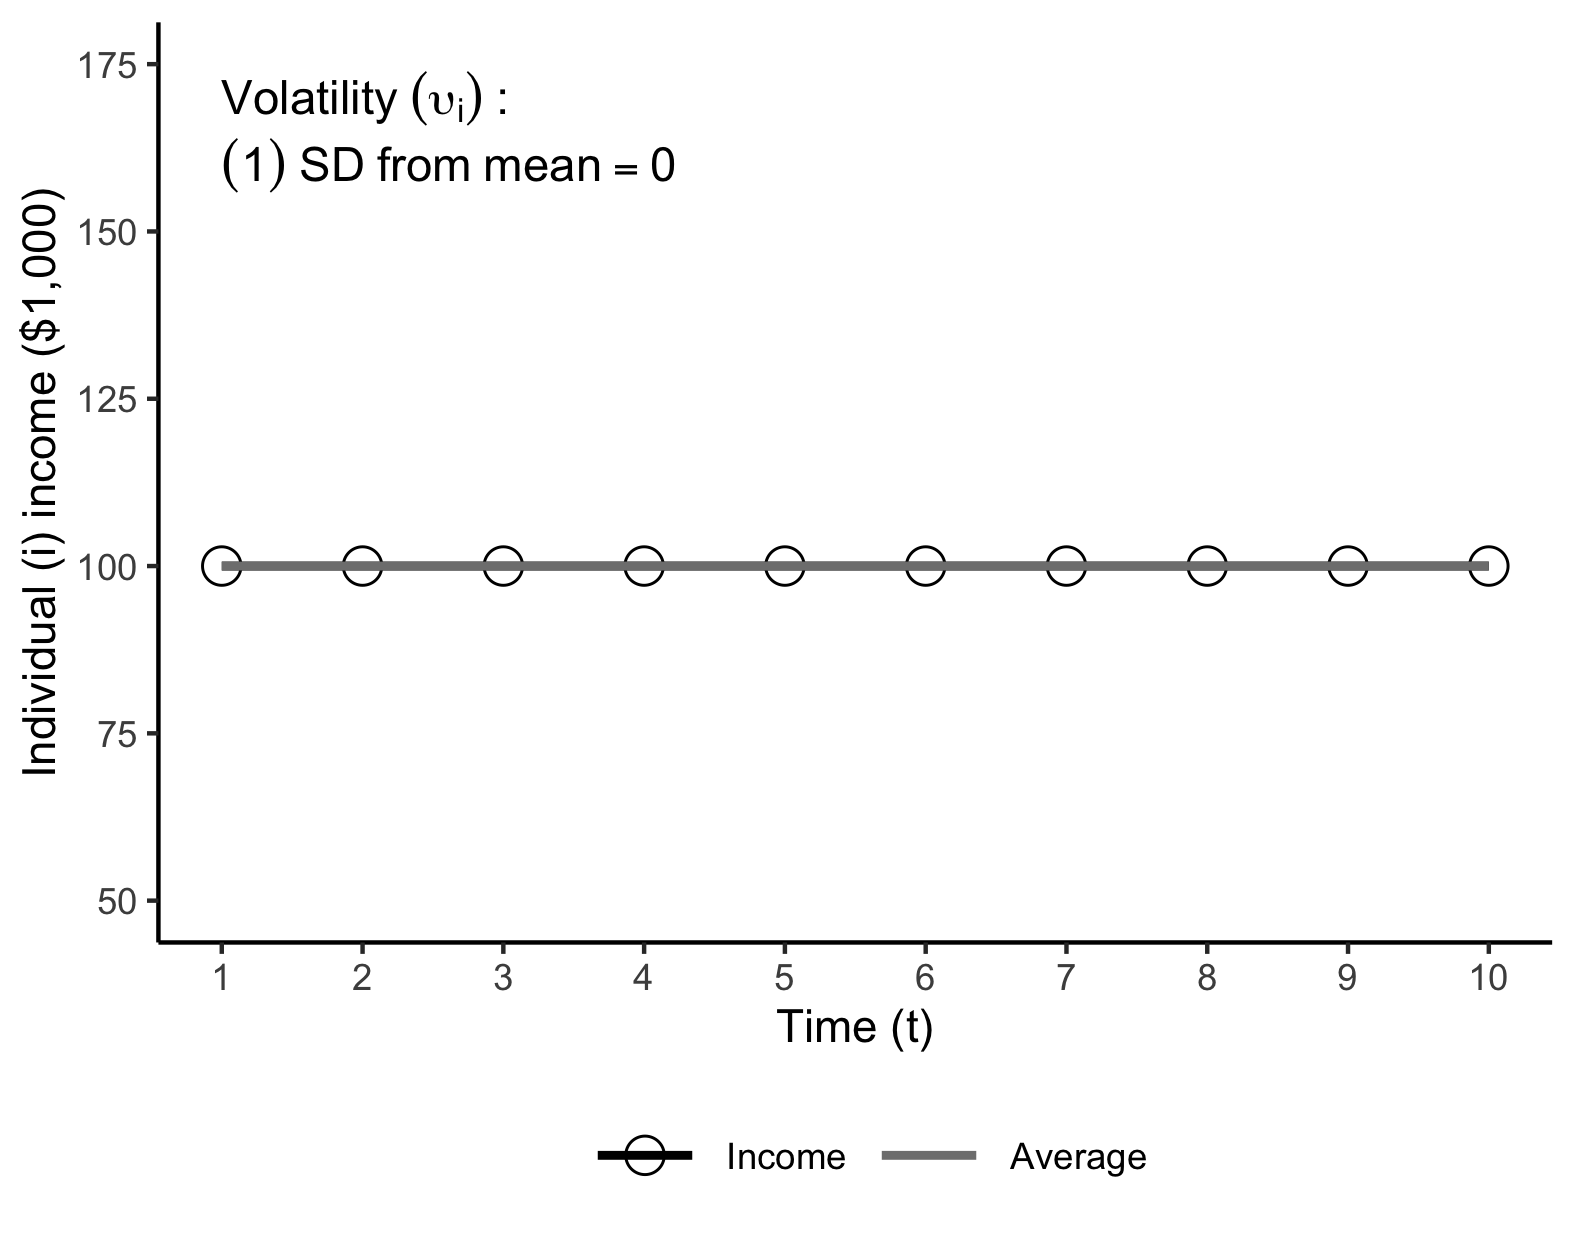
\includegraphics[width=\textwidth]{example_1.png}
        \caption{No income change}
        \label{examples_sub1}
    \end{subfigure}
    \begin{subfigure}[b]{0.45\textwidth}
        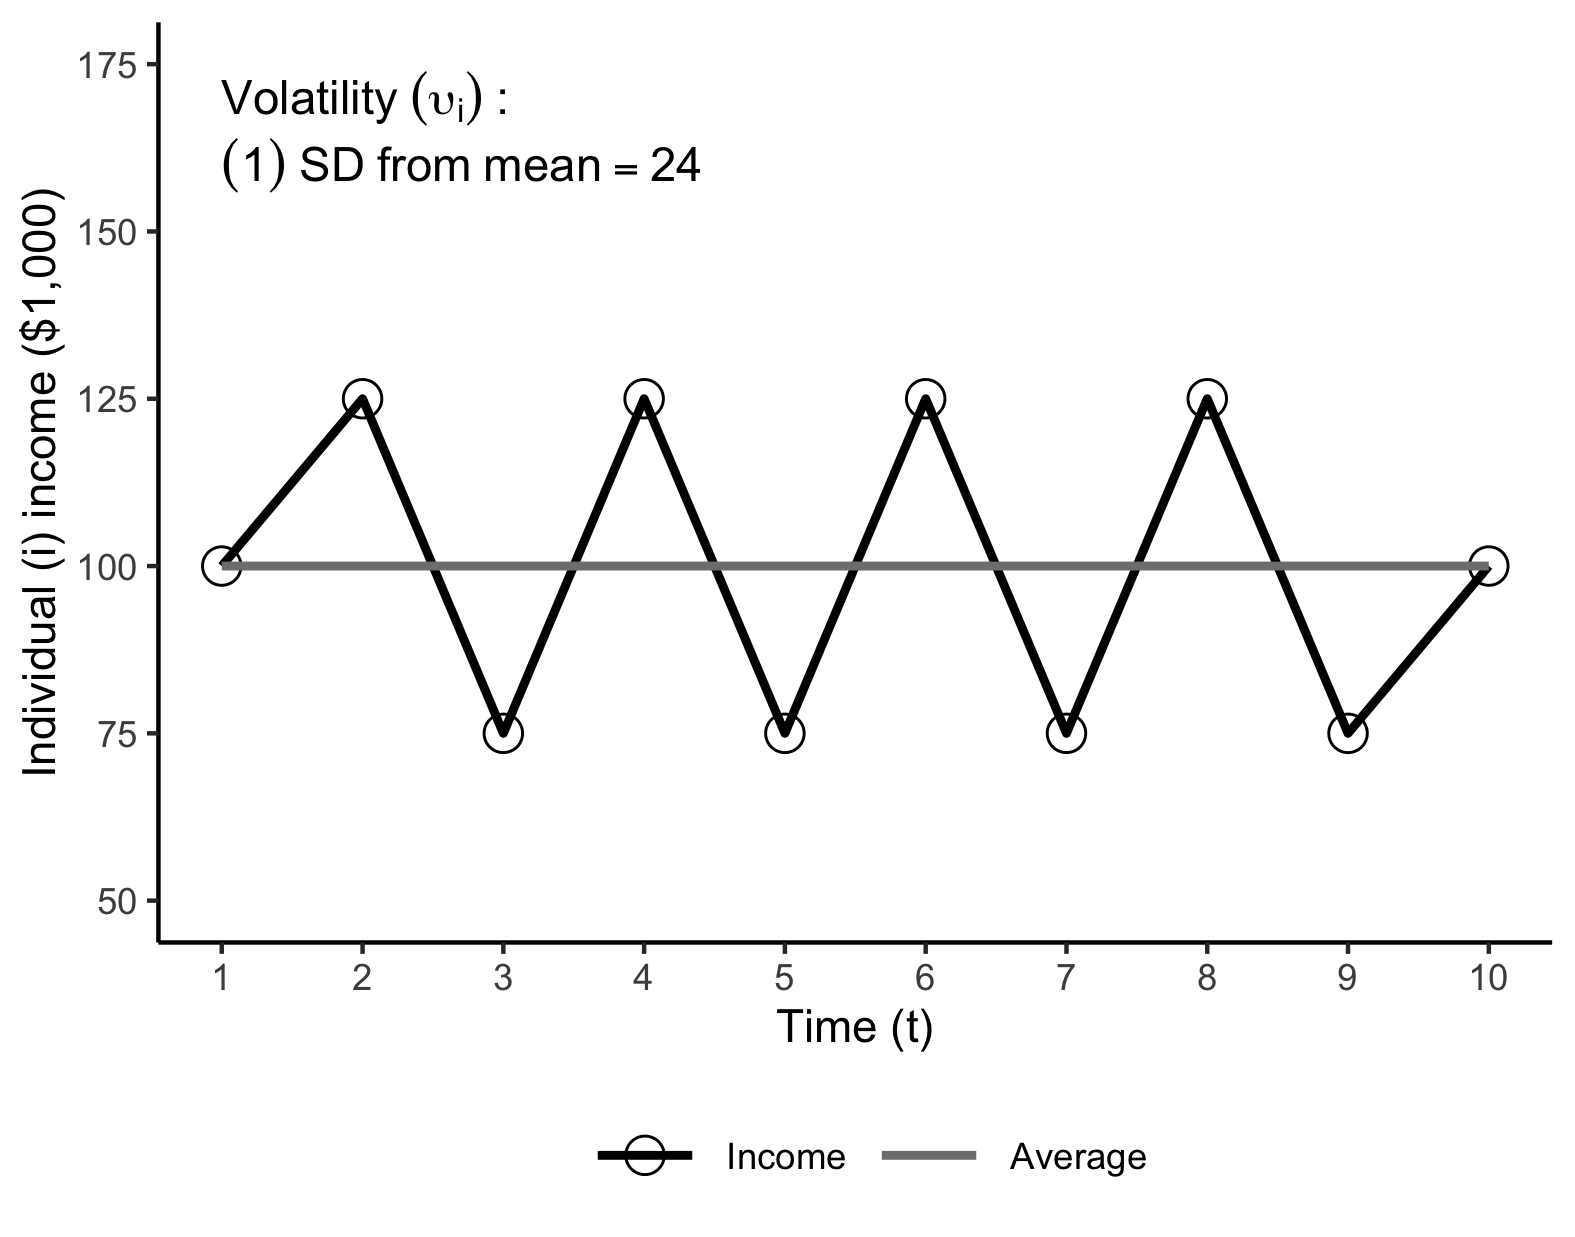
\includegraphics[width=\textwidth]{example_2.png}
        \caption{Mean reverting}
        \label{examples_sub2}
    \end{subfigure}
        \begin{subfigure}[b]{0.45\textwidth}
        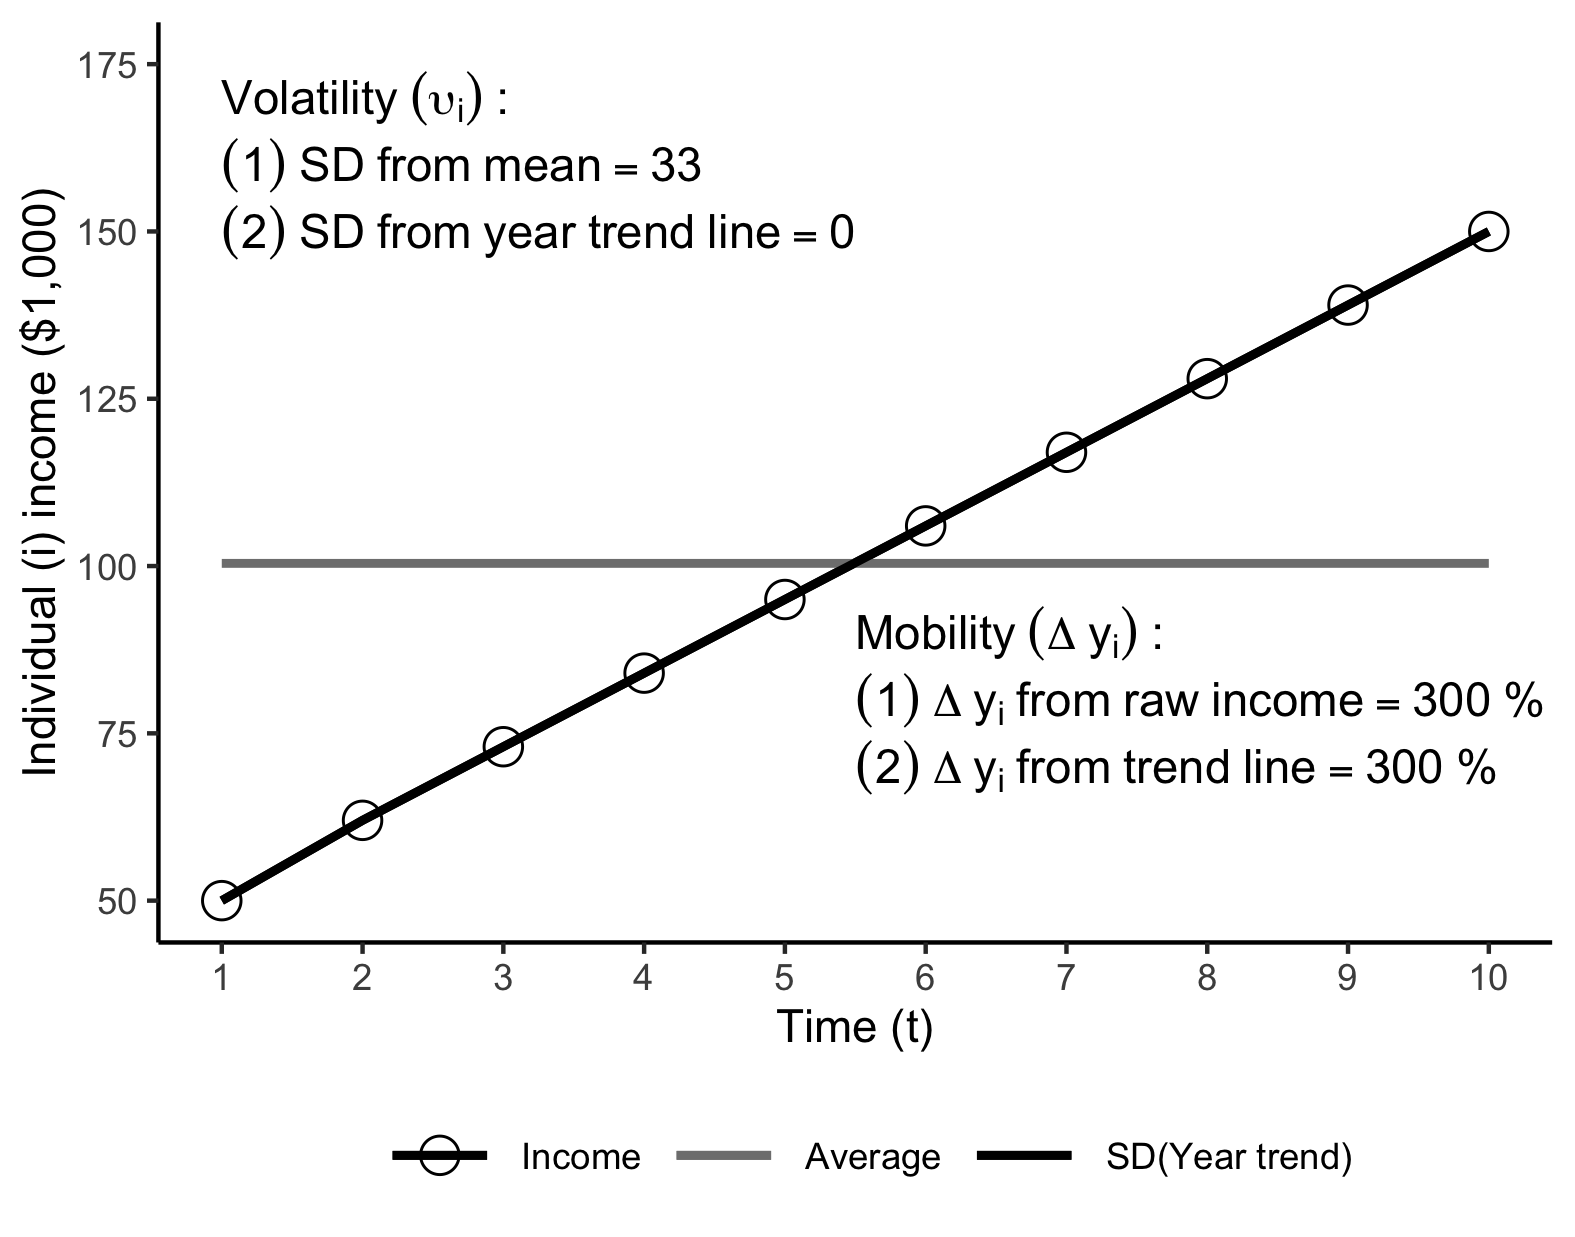
\includegraphics[width=\textwidth]{example_3.png}
        \caption{Linear}
        \label{examples_sub3}
    \end{subfigure}
    \begin{subfigure}[b]{0.45\textwidth}
        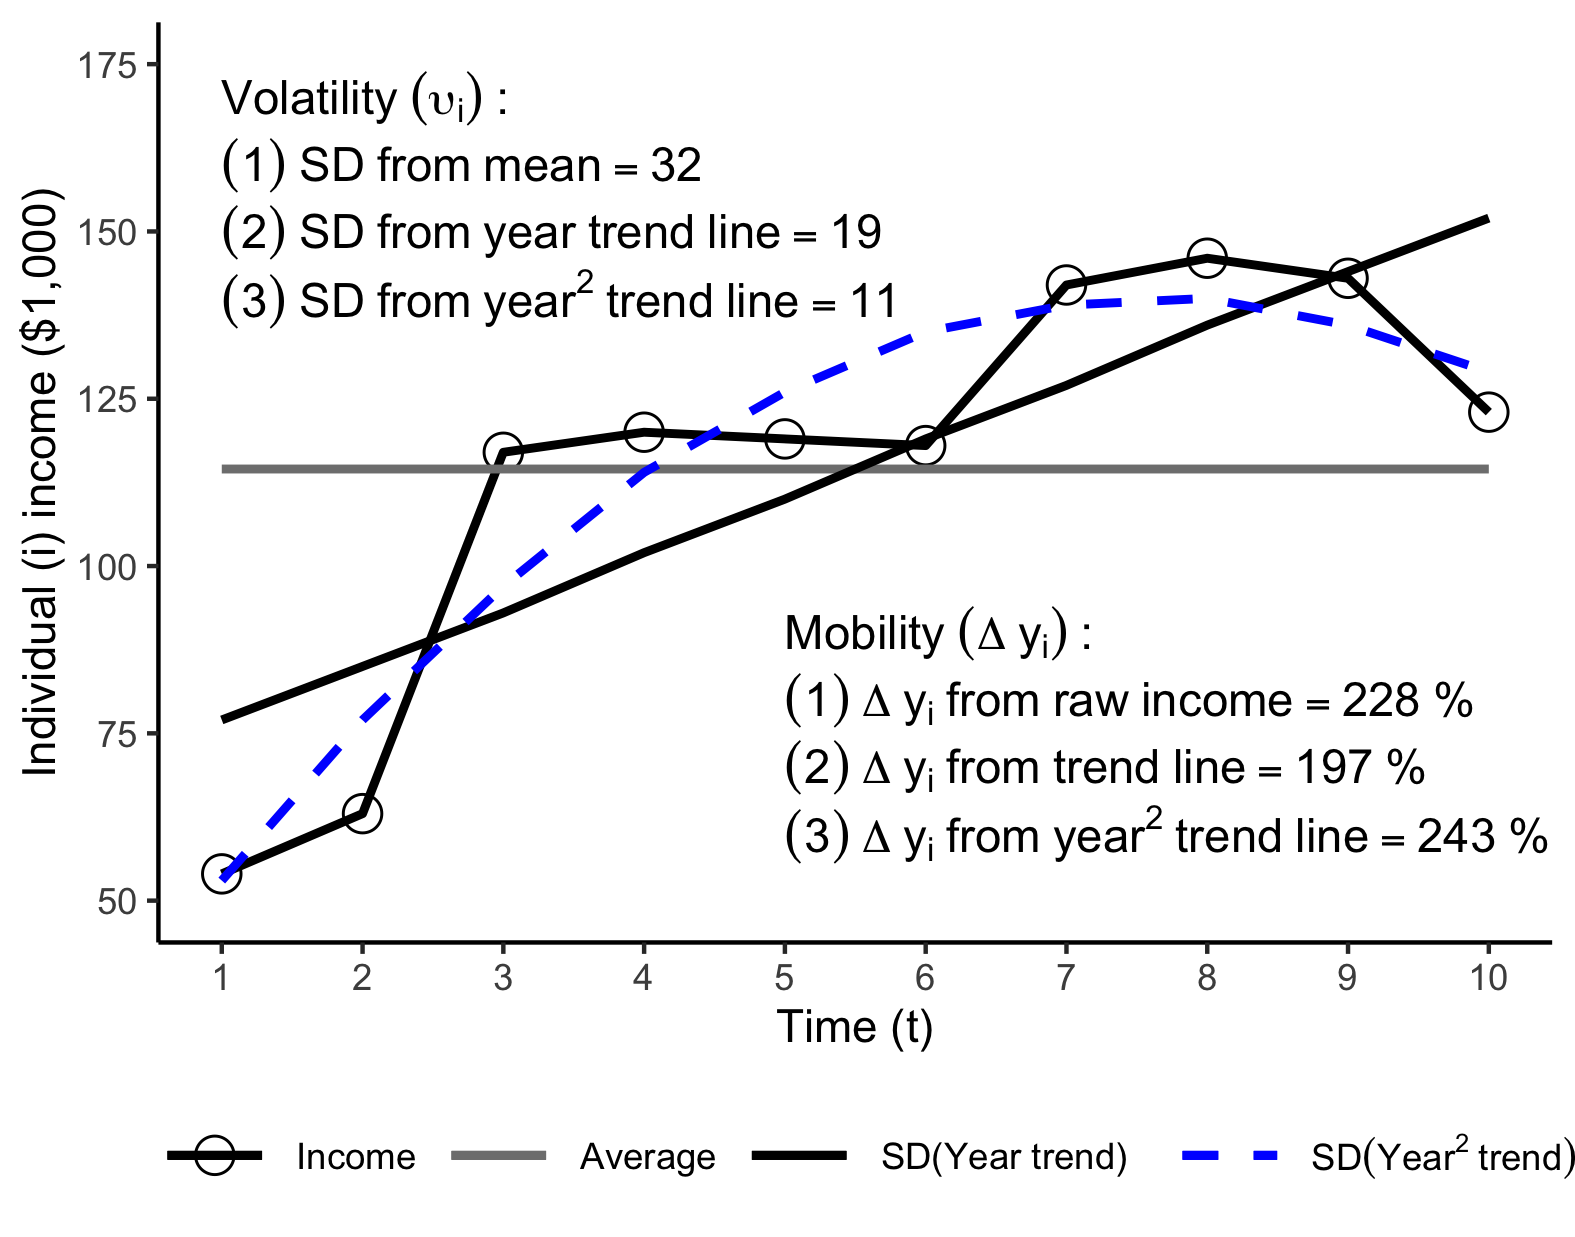
\includegraphics[width=\textwidth]{example_psid.png}
        \caption{Curvilinear}
        \label{examples_sub4}
    \end{subfigure}
\end{sidewaysfigure}

\begin{figure}[htp!]
\centering
\caption{Income volatility over time with different measures of volatility} 
\centering
\resizebox{\textwidth}{!}{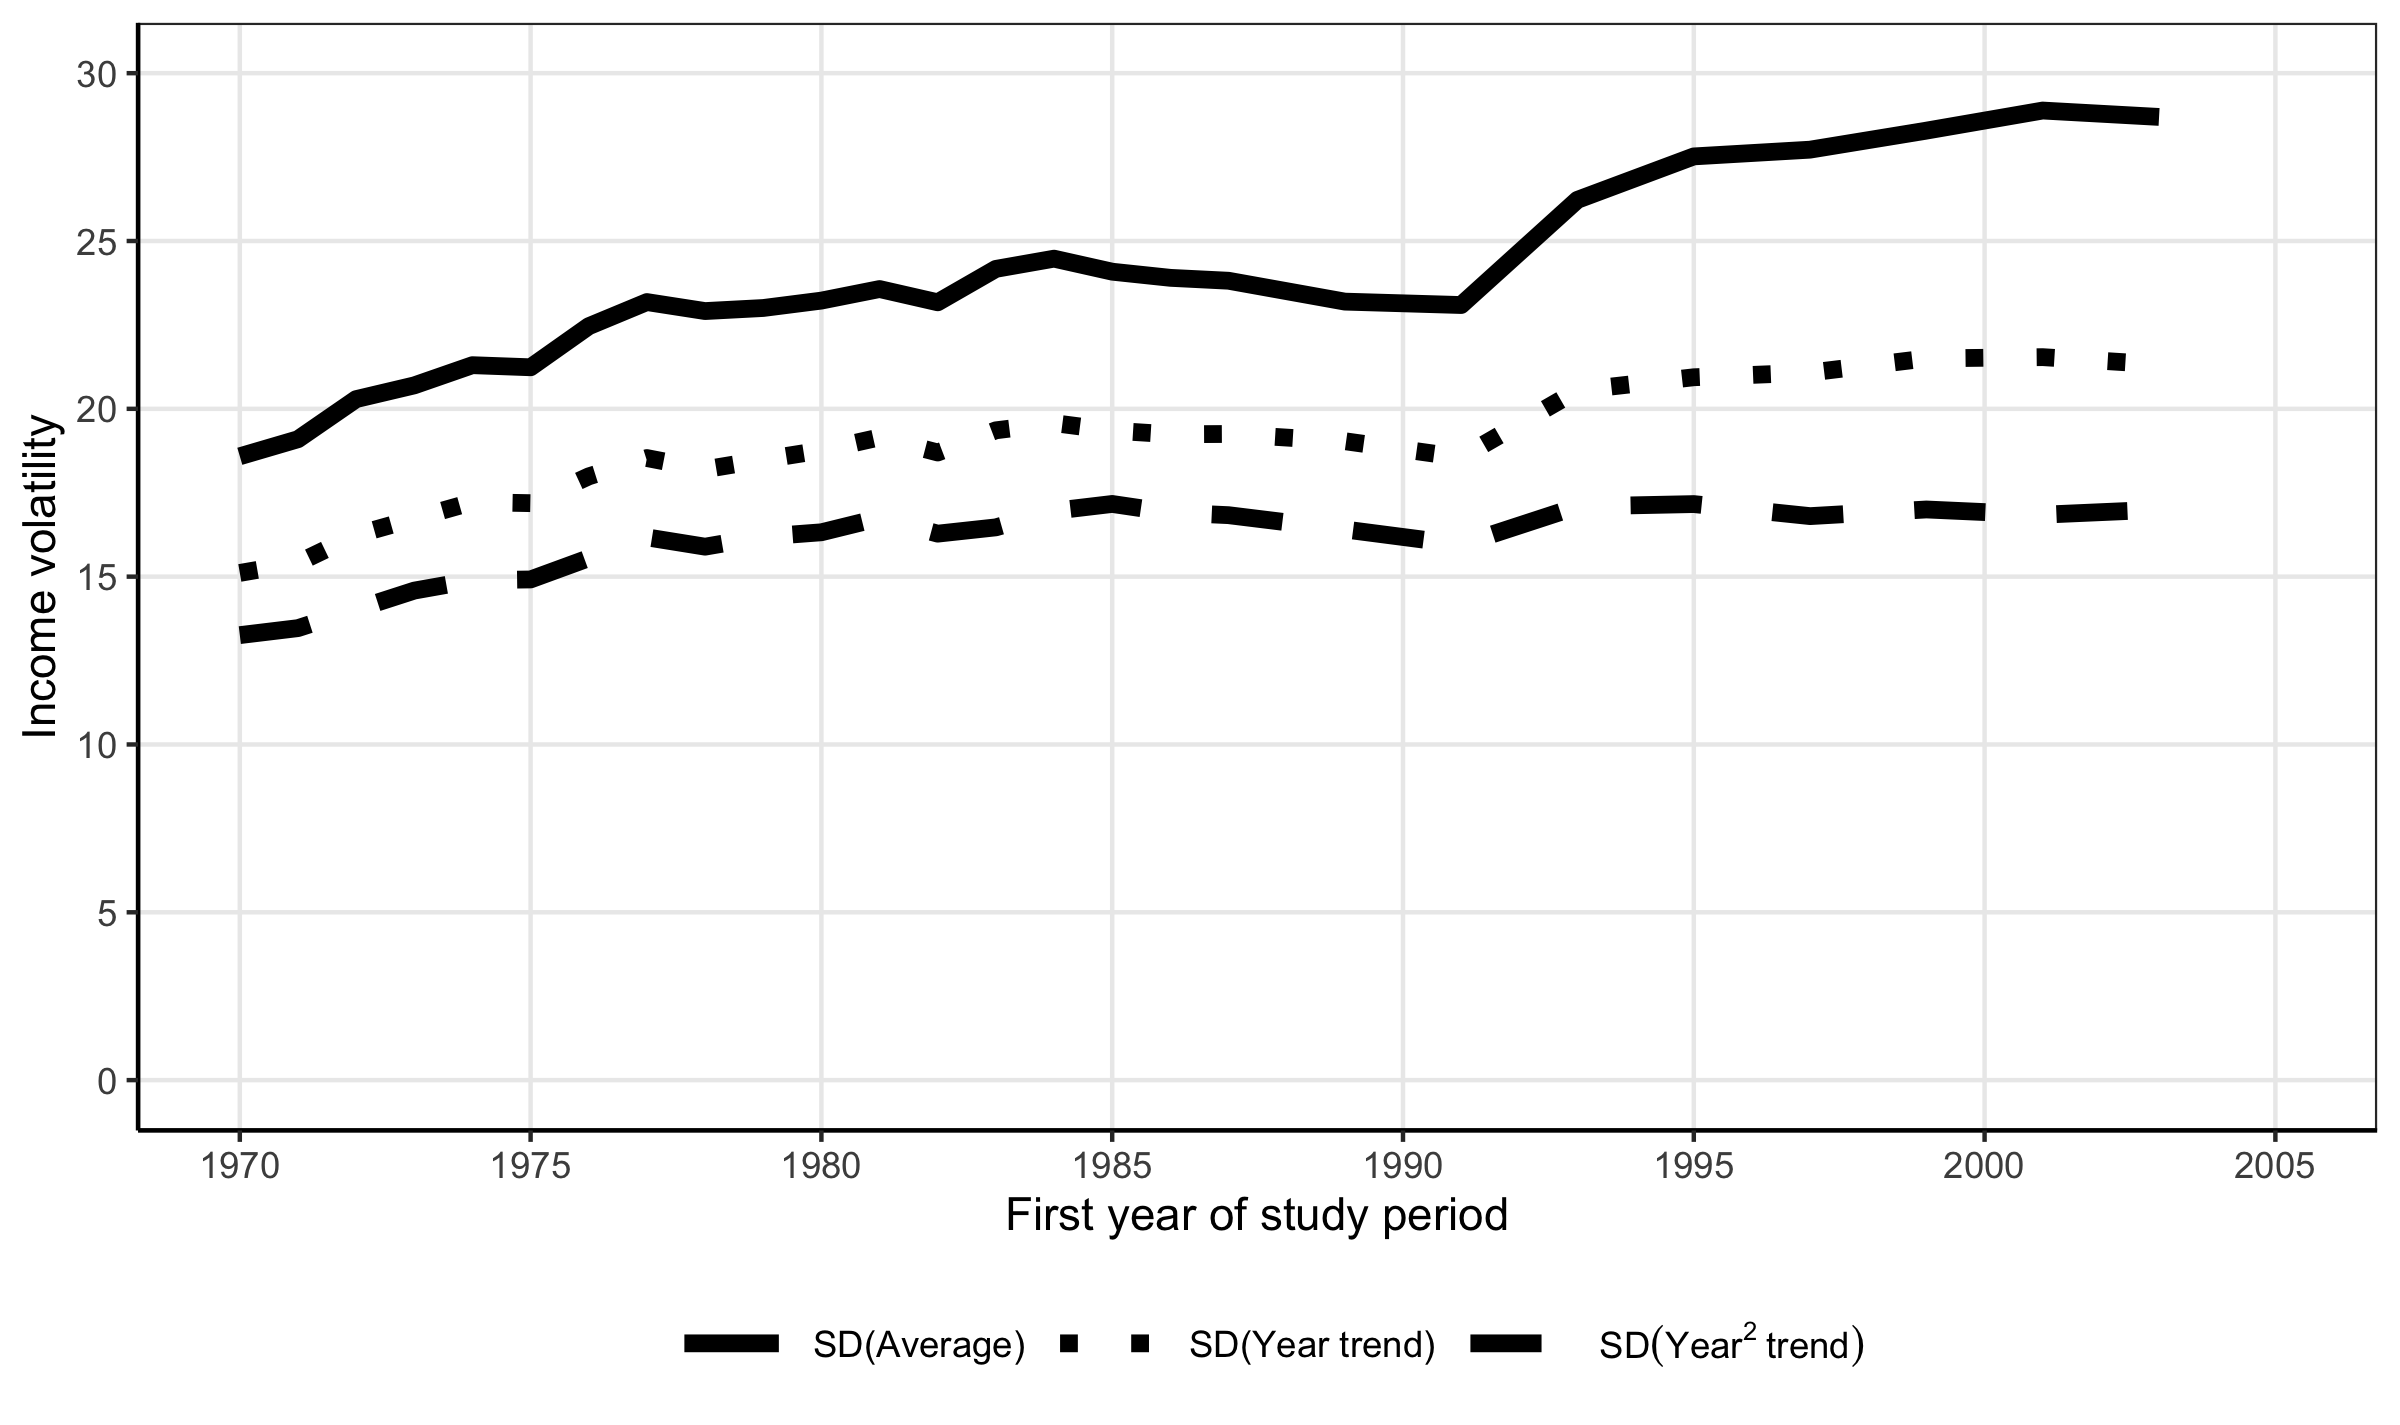
\includegraphics{volatility_graph_src.png}}
\label{volatility_graph}
\end{figure}

\begin{figure}[htp!]
\centering
\caption{Predicted income volatility by income mobility from table \ref{regression}} 
\centering
\resizebox{\textwidth}{!}{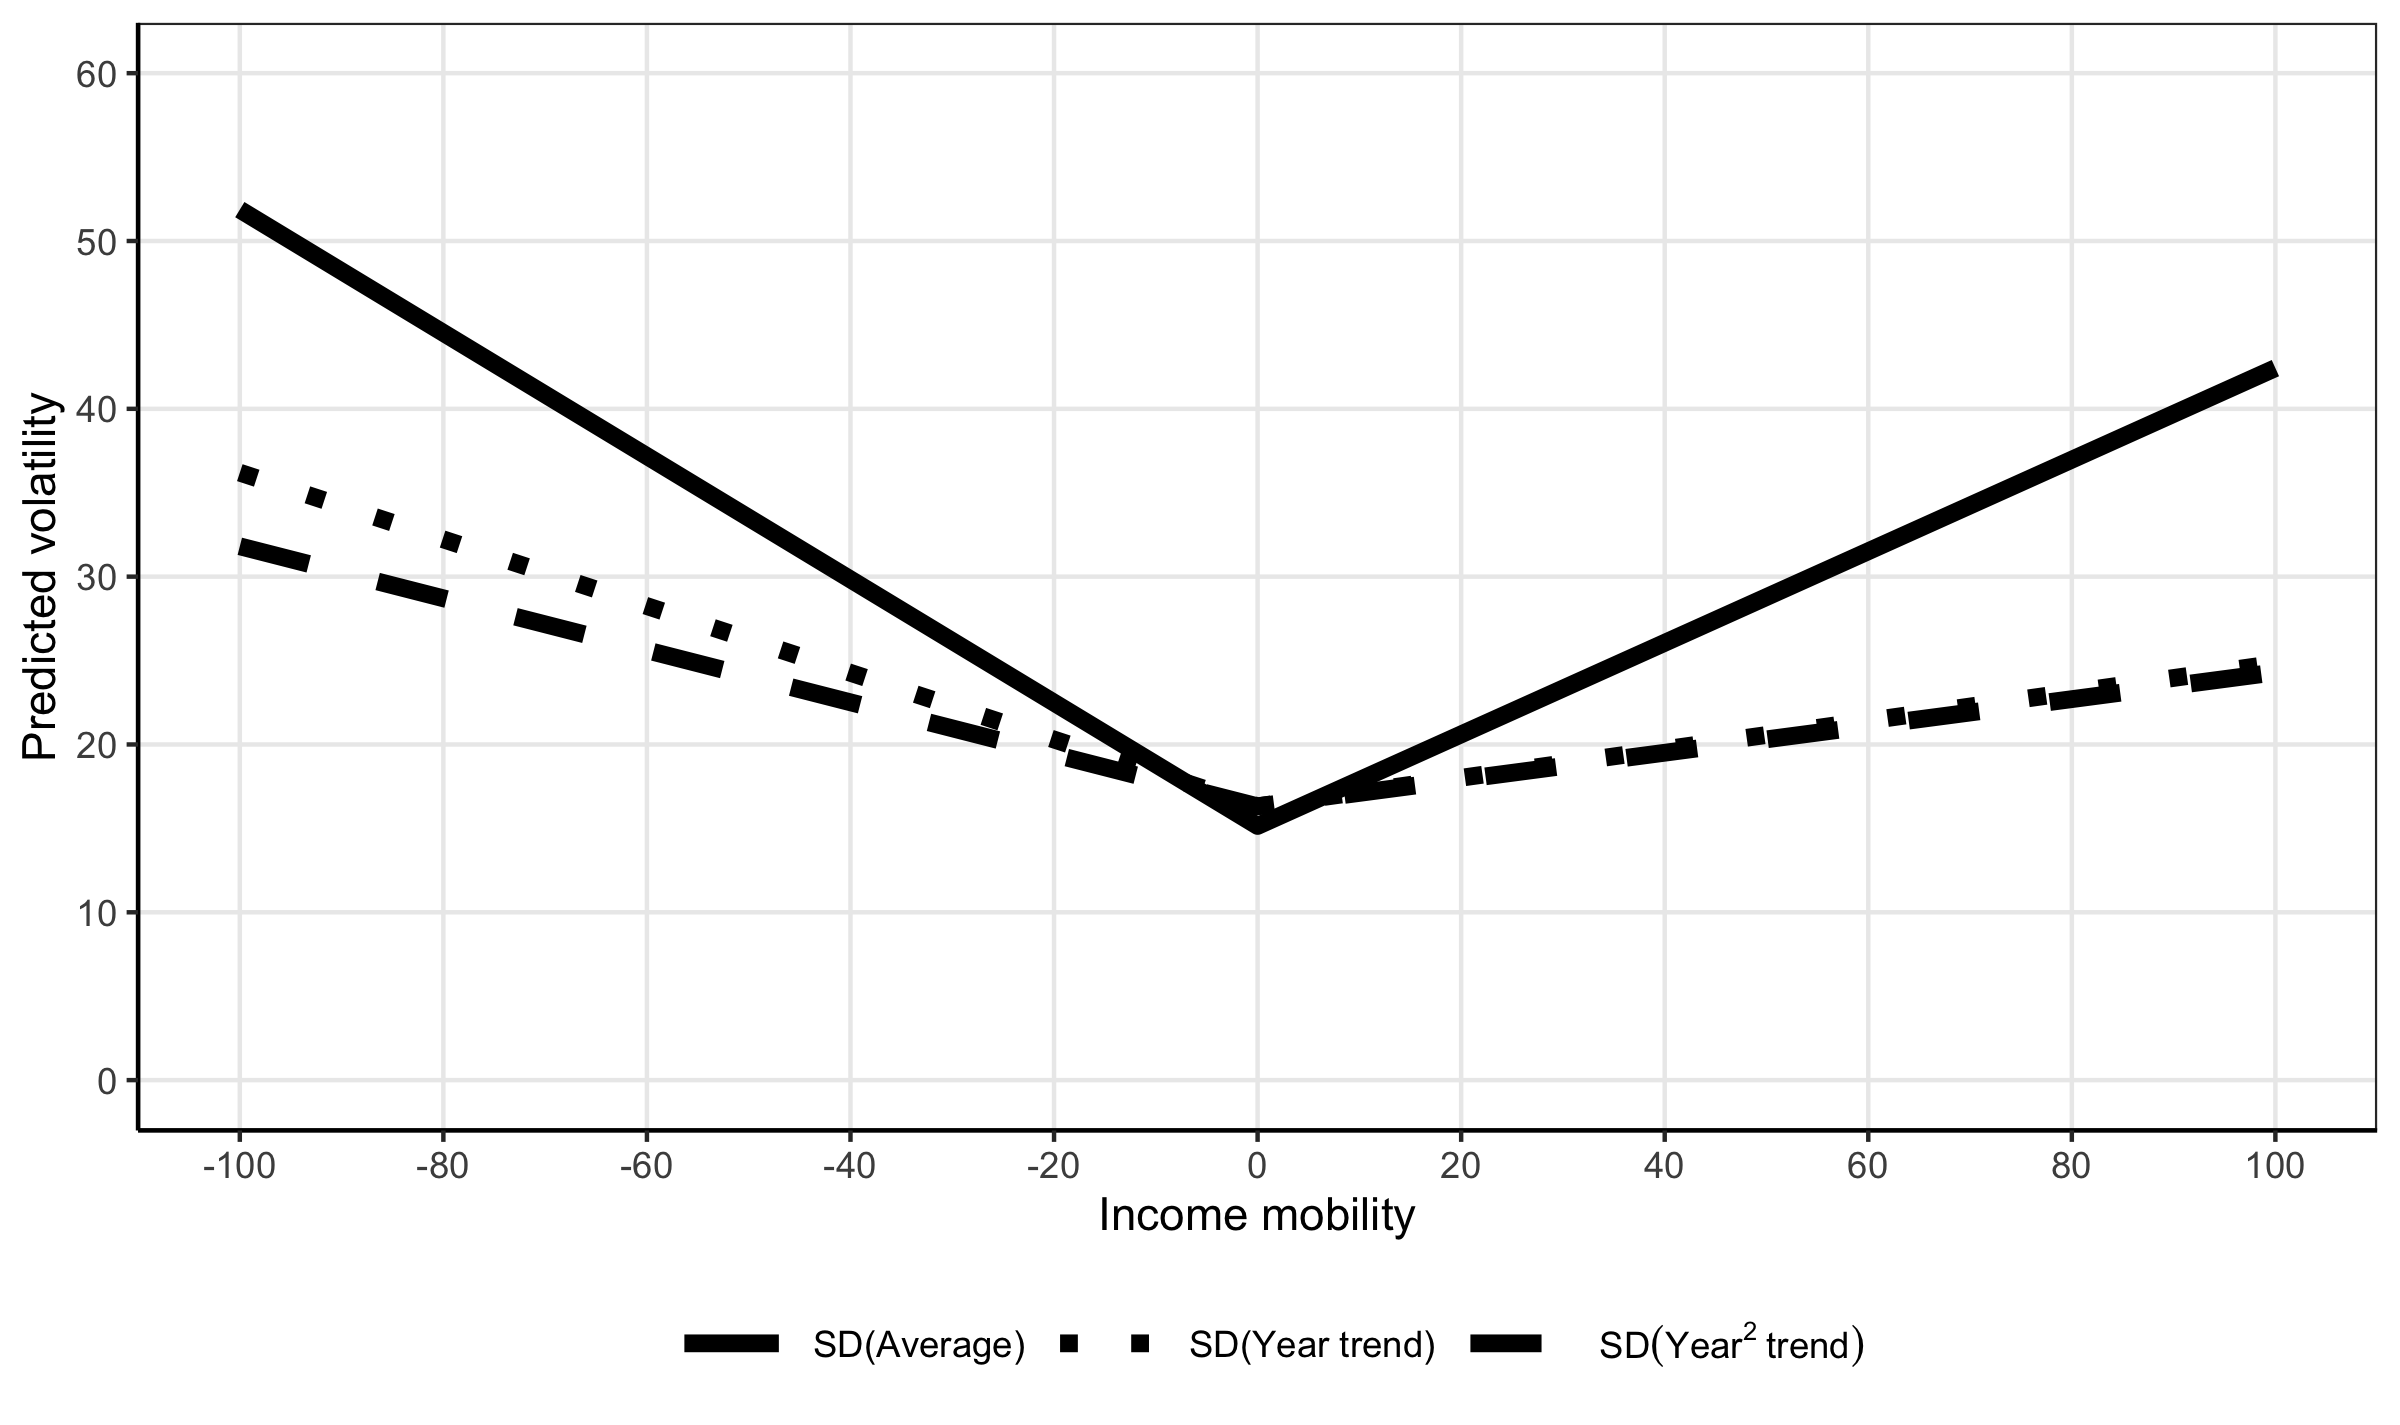
\includegraphics{margins_ind_src_apc_w_o_cube.png}}
\label{margins_mobility}
\end{figure}

%%%%%%%%%%%%%%%%%%%%%%%%%%
%APPENDIX
%%%%%%%%%%%%%%%%%%%%%%%%%%

\clearpage
\appendix
\section{Appendix}
\label{appendix_a}
\setcounter{table}{0}
\setcounter{figure}{0}
\renewcommand*\thetable{\Alph{section}.\arabic{table}}
\renewcommand*\thefigure{\Alph{section}.\arabic{figure}}

We compare the sensitivity of the main findings across a variety of alternative model specifications and sample selections in order to measure the robustness of the results. Without discounting the importance of these issues, the results are qualitatively similar and do not alter the main findings. 

As mentioned earlier, not only are there alternative measures of volatility, but there are also alternative measures of mobility. One is the difference between the beginning and end of a study period in the predicted log of income from the year-adjusted trend line for each individual, as shown in equation \ref{linear}. The other is the difference between average log income in the last two years of a study period and the first two years of a study period, as shown in equation \ref{average}. In contrast to the examples described in figure \ref{examples}, the first and last two years are averaged in order to get a more stable measure of income start and end during a study period. 

Another critique is that the models may not appropriately account for the age-earnings profiles. A cursory knowledge of the way earnings evolve over time would not only suggest that young individuals have an upward earnings trend and older individuals have a downward earnings trend, but also the trend of younger individuals is likely to be smooth while the trend of older individuals is likely to be volatile. To be consistent with the literature, the income measure used is the residual of year fixed effects within each 11-year study period, but the adjustment may not be sufficient to capture the age specific earnings profiles. Therefore, we have replicated with the results using a sub-sample of young, middle, and older individuals. 

As mentioned in the data section, the sample is an unbalanced panel comprised of multiple, overlapping 11-year, balanced panels. This raises two major issues: sample weights and econometric models.

First, sample weights are available that may be used to generate population representative results from the the PSID. Following Shin and Solon \citeyearpar{shin_solon_2011}, we use the nationally representative Survey Research Center (SRC) sub-sample of the PSID. While the PSID also includes samples of low-income (SEO sample), immigrant, and Latino households, Shin and Solon raise critical concerns with each of these samples. Weights are available that may be used to generate population representative results from these additional subsamples, but it is not clear that the weights are able to overcome the underlying issues. Using the SRC sample also allows us to avoid the problem of sample attrition in the PSID, which is a particular problem for studies of income volatility that rely on a balanced subsample within each time period \citep{nichols_rehm_2014}. While all of the results presented here use the SRC sample, it is worth noting that the same results were achieved with the inclusion of the low-income (SEO) sample.

Second, the reliance on multiple, overlapping balanced panels also represents a potential challenge with the use of a fixed-effects model. Despite the advantages of a fixed effects model, as discussed earlier, there are disadvantages. A critical concern is that a fixed effects model ignores individuals who are only in the sample in a single, 11-year study period, i.e. `singletons.' Of the 3,560 unique individuals in the sample, there are 478 individuals who are only present in one, 11-year study period, which represents 13\% of the sample. 

Two alternative models are able to address the weakness of the fixed effects models, but not without cost.  One alternative is a pooled ordinary least squares (POLS) regression that includes singletons, but ignores the panel structure completely.  Another alternative is a random effects model. Like a fixed effects model, a random effects model addresses the issue of autocorrelation, but, unlike a fixed effects model, would include singletons. Further, a random effects model could also control for both time-varying and -invarying factors. The disadvantage is that a random effects model assumes that unobserved heterogeneity will not bias the estimates. The assumption of no unobserved heterogeneity is a strong assumption and one of the main reasons why fixed effects models are often preferred over random effects when using panel data. The results presented here are not sensitive to the use of fixed effects, POLS, or random effects models (with or without other, time-varying or -invarying control variables). 

There are also three components of our selection criteria that are not settled in the literature: (1) study period length, (2) income bound (i.e. bottom code), and (3) individual- or family-level income. 

First, there is no uniform agreement on what constitutes a study period. Some use sequential study periods \citep{dynan_etal_2012,shin_solon_2011,nichols_rehm_2014}, others use study periods of four-years \citep{hacker_2006}, nine-years \citep{gottschalk_moffitt_2009}, or five-years \citep{gottschalk_moffitt_1994}. We use an 11-year study period in our analysis. The gain is the ability to create a more representative trend line, especially after 1997. The sacrifice is fewer individuals are included in any given survey period. To address this concern, we have replicated the results using a 7-year study period. 

Second, there is almost no uniform agreement on what is the appropriate lower bound estimate for income. Most studies drop individuals whose income is below \$1 or \$100 in a given year in a given study period of varying years. If the goal is to examine income volatility among individuals whose labor market participation is constant, then this makes sense. However, if the goal is to examine income volatility among all individuals, then there is no reason to drop individuals with zero income in a given year in a given study period. In fact, there is a strong reason to include them: it is individuals who move from zero to non-zero income who may experience the highest levels of volatility. Winship \citeyearpar{winship_2011} notes that a large proportion of rising income volatility is explained by individuals whose incomes move from non-zero to 0 or visa versa. If we add \$100 to every observation, then we can include observations with \$0 income and maintain the structure of the distribution.  The results do not change with the inclusion of 0 earners.

Third, the issue of measuring volatility from individual- or family-level wages is a long standing concern. Initial work on income volatility focused primarily on the individual wages and salary of prime-age (25-54), white, male, heads of households under the traditional notion that the labor market participation of this group is stable, thereby enabling one to isolate income volatility \citep{gottschalk_danziger_1998}. While the economic position of the household was no longer determined by the male head as more women entered the labor market \citep{diprete_mcmanus_2000}, evidence using the total family income mirrors the evidence at the individual-level. Aggregate levels of volatility are lower, as one would expect, but the rate of increase is similar \citep{gittleman_joyce_1999,dynan_etal_2012}. While legitimate reasons exist why one would prefer to choose one or the other without negating the value of the alternative, we use wages and salary of individuals in order to engage with the longest strain of literature in the sub-field. However, qualitatively similar results are found if we use total family income.

Below, we detail the various alternative model and sample specifications used in tables \ref{regression_sensitivity_avg}, \ref{regression_sensitivity_lin}, and \ref{regression_sensitivity_clin}.

\begin{tabular*}{\textwidth}{@{\extracolsep{\fill}}l l p{10cm}}
\\[-1.8ex]\hline 
\hline \\[-1.8ex] 
Model & Label & Description \\ \hline
1 & From Table \ref{regression}  & Mobility is from the year$^2$-adjusted trend: $\Delta \hat{y}_{0pi} = \hat{y}_{pi,t=N} - \hat{y}_{pi,t=1}$ if $\hat{y}_{pit} = \beta_0 + \beta_{1} T + \beta_{2} T^2$ and $p$ is study period, $i$ is individual, and $ t $ is year. \\
2 & Alt. Mobility 1     &  Mobility is from year-adjusted trend: $\Delta \hat{y}_{0pi} = \hat{y}_{pi,t=N} - \hat{y}_{pi,t=1}$ if $\hat{y}_{pit} = \beta_0 + \beta_{1} T$ and $p$ is study period, $i$ is individual, and $ t $ is year. \\
3 & Alt. Mobility 2     & Mobility is  from unadjusted trend: if $\Delta y_{0pi}$ = difference between average income (LN) in the last 2 years of a study period and the first 2 years of a study period.\\
4 & RE                  & Random effects model \\
5 & POLS                & Pooled Ordinary Least Squares model \\
6 & Biannual            & All 11-year study periods only include data from every other year in order to be consistent with the biannual structure of the PSID after 1997.  For example, the 11-year study period between 1970 - 1980, includes data 6 periods of time (1970, 1972, 1974, 1976, 1978, 1980). \\
7 & Household           & Total household income \\
8 & RE w/controls       & Random effects model w/controls for time (in)varying characteristics \\
9 & All wages (Incl. 0) & Includes \$0 wages from income and salary by adding \$100 to all wages in order to maintain the distribution of income \\
10 & SRC/SEO            & Includes both SRC (population representative) sample and SEO (poverty) oversample  \\
11 & 7yr period         & 7 year study periods (1970 - 1976, 1971 - 1977, \dots, 2005 - 2013) \\
12 & Age (25-34)        & Restricts sample to include only those between 25 - 34 in the first year of an 11-year study period \\
13 & Age (35-44)        & Restricts sample to include only those between 35 - 44 in the first year of an 11-year study period \\
14 & Age (45-54)        & Restricts sample to include only those between 45 - 54 in the first year of an 11-year study period \\
15 & Residual           & Income is the residual from year, education, gender, and race fixed effects \\
\hline 
\hline \\[-1.8ex] 
\end{tabular*}

\clearpage
\begin{sidewaystable}
\caption{Determinants of income volatility, parameter estimates from fixed effects models with alternative specifications (as compared to model 1.C in table \ref{regression})}
\centering
\resizebox{\textwidth}{!}{\input{regression_sensitivity_avg_resid.tex}}
\label{regression_sensitivity_avg}
\end{sidewaystable}

\begin{sidewaystable}
\caption{Determinants of income volatility, parameter estimates from fixed effects models with alternative specifications (as compared to model 2.C in table \ref{regression})}
\centering
\resizebox{\textwidth}{!}{\input{regression_sensitivity_lin_resid.tex}}
\label{regression_sensitivity_lin}
\end{sidewaystable}

\begin{sidewaystable}
\caption{Determinants of income volatility, parameter estimates from fixed effects models with alternative specifications (as compared to model 3.C in table \ref{regression})}
\centering
\resizebox{\textwidth}{!}{\input{regression_sensitivity_clin_resid.tex}}
\label{regression_sensitivity_clin}
\end{sidewaystable}


\end{document}



\end{document}

